\documentclass[10pt]{article}

\usepackage[margin=1in]{geometry}
\usepackage{amsmath,amssymb}
\usepackage{booktabs}
\usepackage{multirow}
\usepackage{graphicx}
\usepackage{xcolor}
\usepackage{hyperref}
\usepackage{url}
\usepackage{xspace}

\newcommand{\method}{CarActGen\xspace}
\newcommand{\artformer}{ArtFormer\xspace}
\newcommand{\placeholder}[2]{
  \begin{center}
  \fbox{\begin{minipage}[c][#2][c]{0.92\linewidth}
  \centering #1
  \end{minipage}}
  \end{center}
}

\title{\textbf{\method}: Function-Aware Multimodal Generation and Learnable Assembly of Interactable Four-Wheel Cars}
\author{Yang Xu 2400011029 \\ https://github.com/mystic-qaq/CarActGen.git}
\date{}

\begin{document}
\maketitle

\begin{abstract}
Generating articulated 3D assets has moved beyond static shape synthesis: practical assets should expose meaningful parts, support intuitive control, and remain compatible with downstream interaction. Existing articulated-object generators such as \artformer demonstrate that part-level latent diffusion can produce diverse movable furniture, but directly transferring this paradigm to cars is non-trivial. Cars have a simple but strict functional topology: a static body and four rotating wheels. A model must therefore preserve small wheel components, place wheel anchors consistently with the generated body, and accept both semantic and visual design conditions.

We present \method, a function-aware extension of the \artformer generation pipeline for four-wheel car assets. We build a small but fully processed car dataset with 484 shapes, 2,420 separated part meshes, per-part textual descriptions, rendered sketch conditions, function labels, bounding boxes, and wheel-anchor metadata. On top of this data, we redesign the SDF VAE as a function-aware latent interface with function identifiers, FiLM conditioning, function-specific reconstruction weights, plane-feature reconstruction, eikonal regularization, and adaptive SDF sampling. We further redesign the latent diffusion module into a multimodal object denoiser with part-local text conditioning, object-level sketch conditioning, branch-specific prediction heads, function-aware loss weighting, and text--image fusion. Finally, we add LayoutNet, a clean-split supervised layout module that predicts the fixed five-part body/wheel boxes and wheel joint origins from generated part latents and multimodal conditions. Both the original and PartLocal diffusion models still fail the strict watertight four-wheel validity test, but PartLocal improves body geometry and exposes wheel topology as the remaining bottleneck; LayoutNet reduces held-out pivot error from $0.08241$ for a train-mean layout to $0.01751$ and raises wheel-box IoU from $0.61045$ to $0.91594$. We also provide a lightweight interactive viewer for inspecting generated body and wheel parts with LayoutNet or anchor-only assembly modes.
\end{abstract}

\section{Introduction}

\ 

3D generative models are increasingly expected to produce assets that can be used, edited, and animated, not only viewed as static geometry. Neural implicit models and diffusion models have made rapid progress in synthesizing shapes from latent codes, text, images, and sketches. However, many generated 3D objects remain monolithic meshes. For applications such as downstream simulation like CFD (sometimes we need set rotating wheels explicitly), game asset creation, design prototyping, and embodied AI, the useful output is often a structured object: parts should be separated, part semantics should be recoverable, and articulated components should support predictable motion.

Articulated 3D generation is therefore a natural next step. \artformer showed that a pipeline combining part-level SDF autoencoding, latent diffusion, and an articulation-aware transformer can generate diverse articulated objects such as cabinets, drawers, and lamps. This is an attractive starting point for vehicle generation because a car also has repeated movable components. Yet cars are not simply another furniture category. Furniture articulation is often category-dependent and may involve hinged panels, sliding drawers, or handles. Four-wheel cars instead have a compact and rigid functional structure: one static body and four rotating wheel supports. This simplicity makes the task appear easier, but in practice it creates a different failure mode. The body is large and visually dominant, while the wheels are small, repeated, thin, and topologically fragile. A generation model can obtain good global appearance while still failing the core functional requirement if a wheel is missing, fragmented, fused to the body, or decoded outside the valid latent region.

This paper studies how to adapt the \artformer paradigm to this car-specific setting. Our goal is not only to generate plausible car-shaped geometry, but to generate a structured asset with a separated body, four wheel parts, part boxes, and wheel anchors that support rotation in visually plausible positions. We call the resulting system \method. The core design choice is to treat function and layout as first-class signals throughout the pipeline. Instead of asking a single part VAE, a single diffusion model, and a fixed assembly template to implicitly solve body/wheel differences, we provide function identifiers and function-aware conditioning at the VAE and diffusion stages, then predict a fixed-schema car layout for final assembly.

Our contributions are:
\begin{itemize}
    \item We construct a processed car generation dataset with 484 shapes, each decomposed into a fixed five-part topology: body shell, front-left wheel, front-right wheel, rear-left wheel, and rear-right wheel. The dataset includes 2,420 part meshes, function labels, per-part text prompts, rendered sketch montages, and DINOv2 sketch embeddings.
    \item We introduce a function-aware SDF VAE for car parts. The model augments the \artformer/GenSDF-style plane-feature autoencoder with function identifiers, latent-space FiLM modulation, optional decoder FiLM, function-specific SDF loss weights, plane reconstruction, eikonal regularization, and function-adaptive sampling.
    \item We redesign the latent diffusion module for multimodal car generation. Our PartLocal object denoiser combines per-part text, object-level sketch features, function and position embeddings, branch-specific denoising heads, function-aware loss weighting, and a text--image agreement loss.
    \item We introduce LayoutNet for functional assembly. Given generated part latents plus text/sketch conditions, LayoutNet predicts the body box, four wheel boxes, and four wheel pivots, replacing source-bounding-box assembly in the final generation path. We also keep a PointNet wheel-anchor predictor as an anchor-only ablation.
    \item We provide quantitative evidence that the redesigned model is better understood as a diffusion-compatible latent interface rather than a uniformly stronger VAE reconstructor. Under a clean split audit, the function-aware VAE greatly reduces plane-feature reconstruction error, while strict diffusion validity remains limited by wheel topology.
    \item We implement a simple browser-based viewer for qualitative inspection of generated car assets, including separated body and wheel meshes, LayoutNet layout metadata, and anchor-only assembly ablations.
\end{itemize}

\section{Related Work}

\paragraph{Neural 3D Shape Representations.}
Implicit neural representations such as DeepSDF~\cite{park2019deepsdf} and Occupancy Networks~\cite{mescheder2019occupancy} model 3D shapes as continuous fields, enabling reconstruction at arbitrary resolution. GenSDF~\cite{chou2022gensdf} uses plane features and a variational latent space to support generative modeling of SDFs. \artformer adopts this style of part-level SDF autoencoding as the first stage of its articulated-object pipeline. \method retains this useful implicit representation, but modifies the latent interface to account for car part functions.

\paragraph{3D Generative Models.}
Recent 3D generation methods use GANs, diffusion models, or score distillation to synthesize objects from text, images, or latent noise~\cite{poole2022dreamfusion,lin2023magic3d,jun2023shap-e,nichol2022point-e}. These methods emphasize visual plausibility and diversity, but many generate static shapes or single meshes. In contrast, \method focuses on structured car assets in which wheel parts must remain separated and functionally meaningful.

\paragraph{Articulated and Interactable Objects.}
PartNet~\cite{mo2019partnet}, PartNet-Mobility/SAPIEN~\cite{xiang2020sapien}, and related datasets expose movable object parts and joint metadata, motivating models that reason about object structure rather than only surface geometry. \artformer~\cite{artformer2025} is the most direct baseline for our work: it generates articulated objects by combining an SDF autoencoder, a diffusion model over part latents, and an articulation transformer. We use \artformer as both an architectural reference and an experimental baseline. Our setting differs because the target class is not a broad furniture collection but a constrained car topology with repeated rotating wheels. This changes the key bottleneck from category-level articulation diversity to robust preservation of small repeated functional components.

\paragraph{Multimodal Conditioning.}
Text encoders such as T5~\cite{raffel2020t5} and visual encoders such as DINOv2~\cite{oquab2023dinov2} provide strong semantic features for conditional generation. FiLM~\cite{perez2018film} has been widely used to inject conditioning signals into neural networks through feature-wise scale and shift. \method uses text to describe local part appearance and sketch features to capture object-level silhouette and proportion. We find that the fusion design matters: routing all conditions through a global object context is unstable for wheels, while part-local text attention with object-level sketch attention yields far more valid samples.

\section{Task and Data}

\subsection{Problem Definition}

\ 

Given a conditioning signal $c$ consisting of per-part text, an optional object sketch, or both, the model generates a structured car asset
\begin{equation}
    \mathcal{A} = \{(M_i, f_i, b_i, j_i)\}_{i=1}^{5},
\end{equation}
where $M_i$ is a mesh, $f_i$ is a function label, $b_i$ is a bounding box, and $j_i$ is articulation metadata. We use a fixed five-part order:
\begin{equation}
    [\text{body}, \text{front-left wheel}, \text{front-right wheel}, \text{rear-left wheel}, \text{rear-right wheel}].
\end{equation}
The body has function \texttt{static\_root}. Each wheel has function \texttt{rotating\_support} and is assigned a rotation axis and $[0,2\pi]$ rotation range. This fixed topology is intentionally narrower than general articulated-object generation, but it enables direct evaluation of the most important car-specific functional requirement: all four wheels should decode as valid, separated, rotatable components. In addition to generating the five meshes, \method predicts the wheel joint origins. This separates two problems that are easy to conflate: generating a valid wheel mesh, and placing that wheel at a plausible body-conditioned anchor.

\subsection{Dataset Construction}

\ 

We build a small car dataset tailored to the above task. The preprocessing pipeline separates body and wheel geometry, normalizes each part, records bounding boxes and joint metadata, annotates function labels, renders sketch montages, encodes sketches with DINOv2, and stores per-part text prompts. Table~\ref{tab:dataset} summarizes the resulting dataset.

\begin{table}[t]
\centering
\caption{Processed car dataset statistics. Every shape follows the same five-part topology.}
\label{tab:dataset}
\begin{tabular}{lr}
\toprule
Item & Count \\
\midrule
Car shapes & 484 \\
Separated part meshes & 2,420 \\
Shapes with complete five-part topology & 484 \\
Train / validation / test split & 392 / 44 / 48 \\
Per-part text prompt files & 2,420 \\
Sketch montage images & 484 \\
DINOv2 sketch embeddings & 484 \\
\texttt{static\_root} body parts & 484 \\
\texttt{rotating\_support} wheel parts & 1,936 \\
Annotated wheel pivots & 1,936 \\
Symmetric wheel-anchor vectors & 484 \\
\bottomrule
\end{tabular}
\end{table}

The fixed topology is a deliberate modeling assumption. It removes ambiguity about part count and interaction type, allowing us to study whether a generative model can preserve small repeated functional parts. At the same time, it is an important limitation: the current dataset does not cover arbitrary vehicle topologies such as six-wheel vehicles, motorcycles, or openable doors.

\section{Method}

\ 

\method follows a three-stage latent generation and assembly pipeline. First, a function-aware SDF VAE maps each part mesh to a latent code and decodes latent codes back to SDF plane features. Second, a multimodal latent diffusion model generates the five part latents jointly at object level. Third, LayoutNet predicts the fixed car layout, including the body bounding box, four wheel bounding boxes, and four wheel joint origins. The generated latents are decoded into meshes and assembled into an interactable asset using the generated meshes, function labels, predicted boxes, and predicted wheel anchors.

\subsection{Function-Aware SDF VAE}

\ 

The original \artformer VAE encodes a part point cloud into triplane-like features, passes these features through a variational bottleneck, and decodes them into an SDF field. This design is category-agnostic at the part level. For cars, however, body and wheel parts differ strongly in scale, topology, and functional importance. Wheels are small and repeated; body shells are large and dominate global appearance. We therefore introduce function conditioning into the VAE.

Let $P_i$ be the point cloud of part $i$ and $r_i$ its function label. The encoder produces plane features
\begin{equation}
    H_i = E_{\theta}(P_i).
\end{equation}
We concatenate the plane features and modulate them with a learned function embedding $e(r_i)$:
\begin{equation}
    \tilde{H}_i = \mathrm{FiLM}_{\mathrm{in}}(H_i, e(r_i)).
\end{equation}
The VAE maps $\tilde{H}_i$ to a latent $z_i$ and reconstructs plane features
\begin{equation}
    z_i \sim q_{\phi}(z_i \mid \tilde{H}_i), \qquad
    \hat{H}_i = \mathrm{FiLM}_{\mathrm{out}}(D_{\phi}(z_i + s(r_i)), e(r_i)),
\end{equation}
where $s(r_i)$ is a learned function-specific latent shift. The SDF decoder then predicts
\begin{equation}
    \hat{d}_{ij} = F_{\psi}([\mathbf{x}_{ij}, \hat{h}_{ij}], r_i),
\end{equation}
for query point $\mathbf{x}_{ij}$ and interpolated feature $\hat{h}_{ij}$. When decoder FiLM is enabled, $F_{\psi}$ also receives the function embedding through feature-wise modulation.

The VAE training objective is
\begin{equation}
    \mathcal{L}_{\mathrm{VAE}} =
    \lambda_{r_i} \, \|\hat{d}_i - d_i\|_1
    + \mathcal{L}_{\mathrm{KL}}
    + \lambda_{\mathrm{plane}}\|\hat{H}_i - H_i\|_1
    + \lambda_{\mathrm{eik}}\mathcal{L}_{\mathrm{eik}},
\end{equation}
where $\lambda_{r_i}$ is a function-specific SDF weight. The plane reconstruction term keeps the variational bottleneck aligned with the encoder feature space. The eikonal term regularizes the local slope of the decoded SDF field using finite differences:
\begin{equation}
    \mathcal{L}_{\mathrm{eik}} =
    \mathbb{E}_{\mathbf{x},\mathbf{u}}
    \left[\max\left(0, \left|\frac{F(\mathbf{x}+\epsilon\mathbf{u}) - F(\mathbf{x}-\epsilon\mathbf{u})}{2\epsilon}\right| - 1\right)^2\right].
\end{equation}
In practice, this term is only applied during training.

\paragraph{Adaptive Sampling.}
We also modify SDF sampling. Body parts receive more repeated point-cloud observations because they determine global silhouette, while wheel parts use a lower uniform-sample ratio to focus more queries near the surface. In the current configuration, \texttt{static\_root} uses a uniform ratio of $0.25$ and repeat factor $3$, while \texttt{rotating\_support} uses a uniform ratio of $0.20$. This simple function-dependent sampling policy improves the balance between large body surfaces and small wheel structures.

\paragraph{Code-Level Implementation.}
The VAE is implemented in \path{model/FunctionAware/sdf.py}. The central class is \texttt{FunctionAwareSDFAutoEncoder}. Function embeddings, latent FiLM, latent shifts, decoder FiLM, function-specific loss weights, plane reconstruction, and the finite-difference eikonal term are all implemented inside this module. The function vocabulary and automatic label mapping are implemented in \path{model/FunctionAware/functions.py}. The main training configuration used in our final pipeline is \path{configs/1_SDF/train_function_aware_car_adaptive.yaml}.

\subsection{Multimodal Object Diffusion}

\ 

The second stage generates all five part latents jointly. Let
\begin{equation}
    Z = [z_1,\ldots,z_N] \in \mathbb{R}^{N \times 768}, \qquad N=5,
\end{equation}
where each $z_i$ is the flattened latent of a car part. We train a denoising diffusion model~\cite{ho2020ddpm} over normalized latents. The model supports four prediction branches: unconditional, text, image, and text--image. At sampling time we use classifier-free guidance against the unconditional branch; for the original \artformer baseline, we also report DDIM-style accelerated sampling~\cite{song2020ddim}.

\paragraph{Object Tokens and Function Tokens.}
At timestep $t$, noisy latents $Z_t$ are projected to hidden tokens and summed with timestep embeddings, part-position embeddings, and function embeddings:
\begin{equation}
    h_i = W_z z_{i,t} + e_t + e_{\mathrm{pos}}(i) + e_{\mathrm{func}}(r_i).
\end{equation}
An object token is prepended to the sequence. This token summarizes object-level context and allows sketch conditioning to influence all parts.

\paragraph{Routed Fusion Baseline.}
Our first multimodal attempt used a routed design: text and image tokens were compressed into global object contexts, then processed by gated cross-attention blocks. This design is implemented in \path{model/FunctionAware/adaptive_object_routed_multimodal_diffusion.py}. It is useful architectural context, but its early quantitative rows were not produced under the final clean train/validation/test protocol. We therefore treat Routed as a diagnostic design that motivates part-local conditioning, not as a final fair baseline in the main tables.

\paragraph{PartLocal Fusion.}
The final model uses a PartLocal denoiser implemented in \path{model/FunctionAware/adaptive_object_partlocal_multimodal_diffusion.py}. Its key difference is that text conditioning is local to each part, while sketch conditioning remains object-level. The text encoder maps each part's text tokens to local context, and each part token attends to its own text features. The image encoder maps a DINOv2 sketch sequence to object-level visual tokens, and all part tokens can attend to this shared visual context. Separate blocks process text-only, image-only, and fused branches, followed by function-aware output heads:
\begin{equation}
    \hat{v}^{(b)}_i = G_b(h_i, r_i), \qquad b \in \{\mathrm{uncond}, \mathrm{text}, \mathrm{image}, \mathrm{text+image}\}.
\end{equation}
The output heads use function-conditioned scale and shift, so the denoiser can allocate different residual statistics to body and wheel latents.

\paragraph{Training Objective.}
The final PartLocal configuration uses a cosine diffusion schedule with 1,000 timesteps and the $v$-prediction objective. Branch losses are weighted as
\begin{equation}
\mathcal{L}_{\mathrm{diff}} =
w_u \mathcal{L}_u +
w_t \mathcal{L}_t +
w_i \mathcal{L}_i +
w_f \mathcal{L}_f +
w_a \mathcal{L}_{\mathrm{agree}},
\end{equation}
where $\mathcal{L}_{\mathrm{agree}}$ encourages the fused branch to remain close to the average of the text and image predictions. We also apply branch-specific function weights. For example, the text branch upweights \texttt{rotating\_support} to emphasize wheel latents, while the image branch upweights \texttt{static\_root} to emphasize body silhouette. The final training configuration is \path{configs/2_Diff/train_adaptive_object_multimodal_car_sketch_dinov2_partlocal.yaml}.

\subsection{LayoutNet Assembly and Viewer}

\ 

Generated part latents are decoded independently into meshes and then inserted into a fixed five-part car structure. A purely template-based system can use the train-split mean layout, or can copy a source bounding box during evaluation, but neither option is satisfactory for generation: the former ignores wheelbase, track width, and stance variation, while the latter borrows held-out geometry. We therefore train LayoutNet to predict the full fixed-schema layout from generated part latents and the same multimodal conditions used by diffusion.

LayoutNet receives five part latent vectors, pooled part text features, pooled sketch features, function identifiers, and part-position embeddings. Its target vector has 42 dimensions: body center and log-size, four wheel centers relative to the body, four wheel log-sizes relative to the body, and four wheel pivots relative to the body. In notation,
\begin{equation}
    \hat{y}=L_{\omega}(Z,T,I,R), \qquad
    y=[c_b,\log s_b,\Delta c_w,\log \Delta s_w,\Delta p_w].
\end{equation}
After decoding $y$ to physical boxes and pivots, we optionally symmetrize left--right wheel pairs. The training objective is a Smooth-$L_1$ loss on normalized layout targets plus a small prior that discourages invalid front/rear ordering, wrong wheel-side signs, and implausible wheel sizes. LayoutNet is trained only on the clean train split and selected by validation loss. The implementation is \path{experiments/paper_train_layout_net.py}.

For diagnostic comparison, we also train anchor-only predictors that assume the body/wheel boxes are already known and predict only wheel pivots. The strongest anchor-only model is a compact PointNet-style regressor from body surface samples and body-box features; a bounding-box-only MLP is used to test whether body size alone is enough. These anchor-only models are useful ablations, but the final generation path uses LayoutNet because it predicts boxes and pivots jointly. The anchor-only implementation is \path{experiments/paper_train_wheel_anchor_predictor.py}.

Each generated asset stores a \texttt{structure.json} file containing part names, hierarchy, bounding boxes, function labels, mesh paths, wheel joint origins, wheel axes, and rotation limits. When LayoutNet is enabled, the sampler also writes \texttt{layout\_prediction.json}. The viewer loads generated meshes and metadata in the browser, allowing visual inspection of body and wheel separation. The body is static, and each wheel rotates around the lateral axis with a $[0,2\pi]$ range. The same viewer can switch among source/template anchors, anchor-only predictors, and LayoutNet full-layout assembly.

\section{Experiments}

\subsection{Evaluation Protocol}

\ 

We evaluate on the held-out 48-shape test split. For reconstructed or generated meshes, we report part-level validity and geometry metrics:
\begin{itemize}
    \item \textbf{Sample success}: a car sample is successful if all required parts are generated and satisfy the validity checks used by our evaluation script.
    \item \textbf{Watertight rate}: fraction of generated part meshes that are watertight.
    \item \textbf{Wheel one-component rate}: fraction of wheel meshes decoded as a single connected component.
    \item \textbf{Chamfer L1}: normalized bidirectional Chamfer distance between generated and source part surfaces. We report body and wheel groups separately, a part-balanced mean that weights the five parts equally, and a source-surface-area-weighted mean that better reflects the visual dominance of the car body.
    \item \textbf{F-score}: surface F-score at 1\% and 2\% thresholds, with the same body, wheel, part-balanced, and source-surface-area-weighted aggregation choices when applicable.
    \item \textbf{Latent regularity}: statistics of normalized latent magnitudes and nearest-neighbor distance to the training latent distribution.
    \item \textbf{Wheel-anchor accuracy}: pivot L2 error, coordinate MAE, wheelbase error, and front/rear track-width error between predicted and annotated wheel pivots.
\end{itemize}

We compare against three types of baselines. First, we run the original \artformer VAE and diffusion pipeline on our processed car data under the same object-level split discipline: train-only data and latent directories contain only the 392 training shapes, validation is used for checkpoint selection, and the 48 test shapes are used only for final evaluation. Second, we evaluate a clean PartLocal function-aware diffusion rerun using train-only VAE latents and keep older Routed results only as diagnostic context. Third, for assembly we compare LayoutNet with train-mean and canonical layouts, and report PointNet/BBox-MLP wheel-anchor predictors as anchor-only ablations.

\subsection{VAE Reconstruction and Latent Regularity}

\ 

Table~\ref{tab:vae-sdf} compares the original \artformer VAE and our function-aware VAE on SDF query accuracy and latent statistics under the final clean object split. Both rows are evaluated from train-only VAE checkpoints on the same 48 held-out test cars. The result is intentionally nuanced. The original VAE remains slightly better in raw SDF MAE and uniform sign accuracy. Our model, however, greatly improves the latent-to-plane interface: plane-feature reconstruction error drops from $0.77487$ to $0.01587$, and the extreme saturation rate $|z|>2$ drops from $0.0011$ to $0.0007$. The latent standard deviation and $|z|>1$ rate are comparable rather than uniformly better. This supports a narrower claim: the function-aware VAE is not a stronger standalone reconstructor, but it provides a better aligned plane-feature bottleneck for downstream generation.

\begin{table}[t]
\centering
% Source: /data/yangxu/ArtFormer_training/FunctionAware_CarGeneral_Adaptive/paper_experiments/vae_ablations_clean_20260704/eval_sdf_latent/vae_ablation_sdf_latent_summary.csv
\caption{Fair SDF and latent comparison on 48 held-out shapes, 240 parts. Lower is better for MAE, plane L1, latent scale, and saturation; higher is better for sign accuracy.}
\label{tab:vae-sdf}
\resizebox{\linewidth}{!}{
\begin{tabular}{lrrrrrrr}
\toprule
System & Surf. MAE & Unif. MAE & Unif. sign & Plane L1 & Latent std & $|z|>1$ & $|z|>2$ \\
\midrule
Original \artformer VAE, train-only & \textbf{0.01230} & \textbf{0.25896} & \textbf{0.902} & 0.77487 & \textbf{0.275} & 0.0155 & 0.0011 \\
Function-aware VAE, train-only & 0.01318 & 0.26022 & 0.895 & \textbf{0.01587} & 0.285 & \textbf{0.0146} & \textbf{0.0007} \\
\bottomrule
\end{tabular}
}
\end{table}

Table~\ref{tab:vae-ablation} reports the clean matched VAE diagnostics that are most relevant to the downstream diffusion interface. We do not use this table to claim that every VAE modification improves raw reconstruction. In fact, source-surface-area weighting makes the trade-off more visible: the full function-aware VAE has worse body-dominated SDF MAE than several simpler variants. The supported conclusion is narrower. Compared with the original \artformer VAE, the function-aware interface greatly reduces plane-feature error and latent outliers. Removing plane reconstruction breaks this interface, while removing adaptive sampling increases latent saturation. Other toggles, such as decoder FiLM and function loss weighting, were mixed in this small clean benchmark and are treated as implementation stabilizers rather than independent ablation wins.

\begin{table}[t]
\centering
% Sources:
% /data/yangxu/ArtFormer_training/FunctionAware_CarGeneral_Adaptive/paper_experiments/vae_ablations_clean_20260704/eval_sdf_latent/vae_ablation_sdf_latent_summary.csv
% /data/yangxu/ArtFormer_training/FunctionAware_CarGeneral_Adaptive/paper_experiments/vae_ablations_clean_20260704/eval_sdf_latent/vae_ablation_sdf_latent_surface_weighted_summary.csv
\caption{Clean VAE interface diagnostics on 48 held-out shapes, 240 parts. PB is the part-balanced surface MAE over five parts, and SW is the source-surface-area-weighted surface MAE with mean body weight $0.8482$. Lower is better for all columns.}
\label{tab:vae-ablation}
\resizebox{\linewidth}{!}{
\begin{tabular}{lrrrrrr}
\toprule
Variant & PB Surf. MAE & SW Surf. MAE & Plane L1 & Latent std & $|z|>1$ & $|z|>2$ \\
\midrule
Original \artformer VAE & 0.01230 & 0.01075 & 0.77487 & 0.275 & 0.0155 & 0.0011 \\
Full function-aware & 0.01318 & 0.01468 & 0.01587 & 0.285 & 0.0146 & 0.0007 \\
No adaptive sampling & 0.01228 & 0.01066 & 0.02067 & 0.315 & 0.0214 & 0.0022 \\
No plane reconstruction & 0.01278 & 0.01296 & 0.32179 & 0.283 & 0.0156 & 0.0007 \\
\bottomrule
\end{tabular}
}
\end{table}

\subsection{Generated-vs-Source Geometry}

\ 

Table~\ref{tab:diff-geometry} compares generated geometry with the source test shapes for the clean reruns. Because both fair diffusion pipelines fail the strict watertight wheel-validity test, these geometry numbers should be read as surface-similarity evidence on decoded meshes, not as proof of usable assets. A simple part-balanced average is useful for diagnosing the repeated wheel bottleneck, but it is not a faithful visual aggregate for cars: on the held-out test split, the body contributes $84.82\%$ of the source surface area on average. We therefore also report a source-surface-area-weighted aggregate. Under this car-weighted metric, PartLocal text--image generation improves Chamfer from $0.0403$ for the clean original class-mean baseline to $0.0355$, while also improving body Chamfer from $0.0355$ to $0.0297$. Wheel geometry remains the main weakness: the clean original baseline is still marginally better on wheel Chamfer and wheel F@2\%.

\begin{table}[t]
\centering
% Sources:
% /data/yangxu/ArtFormer_training/FunctionAware_CarGeneral_Adaptive/paper_experiments/fair_final_diffusion_geometry_epoch0419_clean_partlocal_20260703/diffusion_geometry_summary.csv
% /data/yangxu/ArtFormer_training/FunctionAware_CarGeneral_Adaptive/paper_experiments/fair_final_diffusion_geometry_epoch0419_clean_partlocal_20260703/diffusion_geometry_surface_weighted_summary.csv
\caption{Generated-vs-source geometry for clean train-only reruns on the same 48 held-out test shapes. PB is the part-balanced mean over the five parts. SW is the source-surface-area-weighted mean, where the body has mean weight $0.8482$ on the test split. Lower Chamfer is better; higher F@2\% is better.}
\label{tab:diff-geometry}
\resizebox{\linewidth}{!}{
\begin{tabular}{lrrrrrrr}
\toprule
System & PB Chamfer & SW Chamfer & SW F@2\% & Body Chamfer & Body F@2\% & Wheel Chamfer & Wheel F@2\% \\
\midrule
Original \artformer, zero $z$ & 0.0610 & 0.0406 & 0.576 & 0.0358 & 0.642 & 0.0674 & 0.206 \\
Original \artformer, class-mean $z$ & 0.0609 & 0.0403 & 0.581 & 0.0355 & 0.649 & \textbf{0.0673} & \textbf{0.206} \\
PartLocal, text, cfg 1.2 & 0.0611 & 0.0376 & 0.659 & 0.0321 & 0.741 & 0.0684 & 0.196 \\
PartLocal, image, cfg 1.2 & 0.0603 & 0.0356 & 0.708 & 0.0298 & 0.800 & 0.0679 & 0.199 \\
PartLocal, text + image, cfg 1.0 & \textbf{0.0601} & \textbf{0.0355} & \textbf{0.711} & \textbf{0.0297} & \textbf{0.802} & 0.0677 & 0.202 \\
PartLocal, text + image, cfg 1.2 & 0.0602 & \textbf{0.0355} & 0.710 & \textbf{0.0297} & 0.801 & 0.0678 & 0.201 \\
\bottomrule
\end{tabular}
}
\end{table}

\subsection{Controlled VAE-to-Diffusion Target Experiment}

\ 

The cleanest downstream compatibility test is to hold the PartLocal diffusion architecture, split, conditions, training budget, and evaluator fixed while changing only the VAE latent target. We train two matched configurations:
\begin{itemize}
    \item \path{partlocal_original_vae_target.yaml}: PartLocal diffusion trained on original \artformer VAE latents.
    \item \path{partlocal_function_aware_target.yaml}: PartLocal diffusion trained on function-aware VAE latents.
\end{itemize}

\ 

Table~\ref{tab:target-compat} reports the controlled result. With the same PartLocal denoiser, the function-aware latent target reaches a lower best validation loss and a slightly lower final validation loss. A small quick-generation sanity check shows similar geometry between the two targets; the original VAE target is slightly better on all/wheel Chamfer in this quick sample, while the function-aware target is slightly better on body Chamfer. We therefore use this table as compatibility evidence rather than a standalone final generation-quality ranking.

\begin{table}[t]
\centering
% Sources:
% /data/yangxu/ArtFormer_training/FunctionAware_CarGeneral_Adaptive/paper_experiments/diffusion_target_compatibility/partlocal_original_vae_target/lightning_logs/version_1/metrics.csv
% /data/yangxu/ArtFormer_training/FunctionAware_CarGeneral_Adaptive/paper_experiments/diffusion_target_compatibility/partlocal_function_aware_target/lightning_logs/version_0/metrics.csv
% /data/yangxu/ArtFormer_training/FunctionAware_CarGeneral_Adaptive/paper_experiments/diffusion_target_compatibility/quick_samples_20260702_144855/geometry/diffusion_geometry_summary.csv
\caption{Controlled VAE-to-diffusion target experiment. Both rows use the same PartLocal architecture, split, conditions, and training budget; only the latent target changes. Quick geometry is measured on a small four-sample text--image sanity set.}
\label{tab:target-compat}
\resizebox{\linewidth}{!}{
\begin{tabular}{lrrrrr}
\toprule
Latent target & Best val loss & Last val loss & Quick all Chamfer & Quick body Chamfer & Quick wheel Chamfer \\
\midrule
Original \artformer VAE latent & 0.37942 & 0.64154 & \textbf{0.0564} & 0.0413 & \textbf{0.0602} \\
Function-aware VAE latent & \textbf{0.33284} & \textbf{0.62665} & 0.0598 & \textbf{0.0388} & 0.0650 \\
\bottomrule
\end{tabular}
}
\end{table}

\subsection{Learnable Layout and Assembly}

\ 

Table~\ref{tab:layout-net} evaluates LayoutNet on the 48 held-out test cars. The train-mean layout is a strong baseline because all objects share the same fixed five-part topology, but it cannot adapt to wheelbase, overhang, stance, and body size. LayoutNet predicts both boxes and pivots, reducing pivot L2 from $0.08241$ to $0.01751$ and increasing wheel-box IoU from $0.61045$ to $0.91594$. This is the final assembly module used by our qualitative viewer and sampling script.

\begin{table}[t]
\centering
% Source: /data/yangxu/ArtFormer_training/FunctionAware_CarGeneral_Adaptive/paper_experiments/layoutnet_clean_20260704/20260704_011316_layout_net_seed20260704/summary.md
\caption{LayoutNet full-layout prediction on the 48-shape held-out test split. LayoutNet predicts body box, wheel boxes, and wheel pivots jointly.}
\label{tab:layout-net}
\resizebox{\linewidth}{!}{
\begin{tabular}{lrrrrrr}
\toprule
Method & BBox center L2 & Wheel center L2 & BBox size MAE & Pivot L2 & BBox IoU & Wheel IoU \\
\midrule
Train-mean layout & 0.07998 & 0.08228 & 0.01997 & 0.08241 & 0.66336 & 0.61045 \\
Canonical layout & 0.09139 & 0.09324 & 0.02362 & 0.09474 & 0.64720 & 0.59538 \\
LayoutNet & \textbf{0.01795} & \textbf{0.01748} & \textbf{0.00501} & \textbf{0.01751} & \textbf{0.92631} & \textbf{0.91594} \\
\bottomrule
\end{tabular}
}
\end{table}

Table~\ref{tab:wheel-anchor} isolates wheel-anchor placement when boxes are already known. The bounding-box MLP performs almost identically to the train-mean template, showing that body size alone is not enough. The PointNet anchor predictor uses body surface evidence and reduces mean pivot L2 error from $0.06405$ to $0.03114$, a 51.4\% relative improvement. This confirms that learned geometry evidence helps joint placement, while Table~\ref{tab:layout-net} shows that the full generation path should predict boxes and anchors jointly.

\begin{table}[t]
\centering
% Sources:
% /data/yangxu/ArtFormer_training/FunctionAware_CarGeneral_Adaptive/paper_experiments/wheel_anchor_predictor/20260702_235953_bbox_mlp_seed20260702/summary.md
% /data/yangxu/ArtFormer_training/FunctionAware_CarGeneral_Adaptive/paper_experiments/wheel_anchor_predictor/20260702_235953_pointnet_anchor_seed20260702/summary.md
\caption{Wheel-anchor prediction on the 48-shape held-out test split. The train-mean template is direct template assembly. Track error is the average of front and rear track-width errors.}
\label{tab:wheel-anchor}
\resizebox{\linewidth}{!}{
\begin{tabular}{lrrrrrrrr}
\toprule
Method & Pivot L2 mean & Pivot L2 med. & Pivot L2 p90 & $x$ MAE & $y$ MAE & $z$ MAE & Wheelbase err. & Track err. \\
\midrule
Train-mean template & 0.06405 & 0.06153 & 0.10374 & 0.05322 & 0.01035 & 0.02362 & 0.07099 & 0.02070 \\
BBox MLP & 0.06394 & 0.05985 & 0.10715 & 0.05333 & 0.01033 & 0.02363 & 0.07361 & 0.02066 \\
PointNet anchor & \textbf{0.03114} & \textbf{0.02761} & \textbf{0.05074} & \textbf{0.02010} & \textbf{0.00259} & \textbf{0.01966} & \textbf{0.02850} & \textbf{0.00519} \\
\bottomrule
\end{tabular}
}
\end{table}

\subsection{Qualitative Results}

\ 

Quantitative metrics do not fully capture whether the car ``looks right''. In particular, reviewers will notice body smoothness, wheel-body separation, stance, silhouette consistency, and whether text or sketch conditioning changes the generated body. Figure~\ref{fig:qualitative-grid} compares the original \artformer pipeline with \method on held-out examples. Across different samples, \method produces visibly smoother body surfaces with fewer local bumps and dents. The tire differences are less obvious in static views because the wheels occupy a much smaller part of the car, but the dominant body region becomes cleaner, so the overall visual quality improves.

\begin{figure}[t]
\centering
\begin{tabular}{@{}ccc@{}}
\textbf{Test 1} & \textbf{Test 2} & \textbf{Test 3} \\
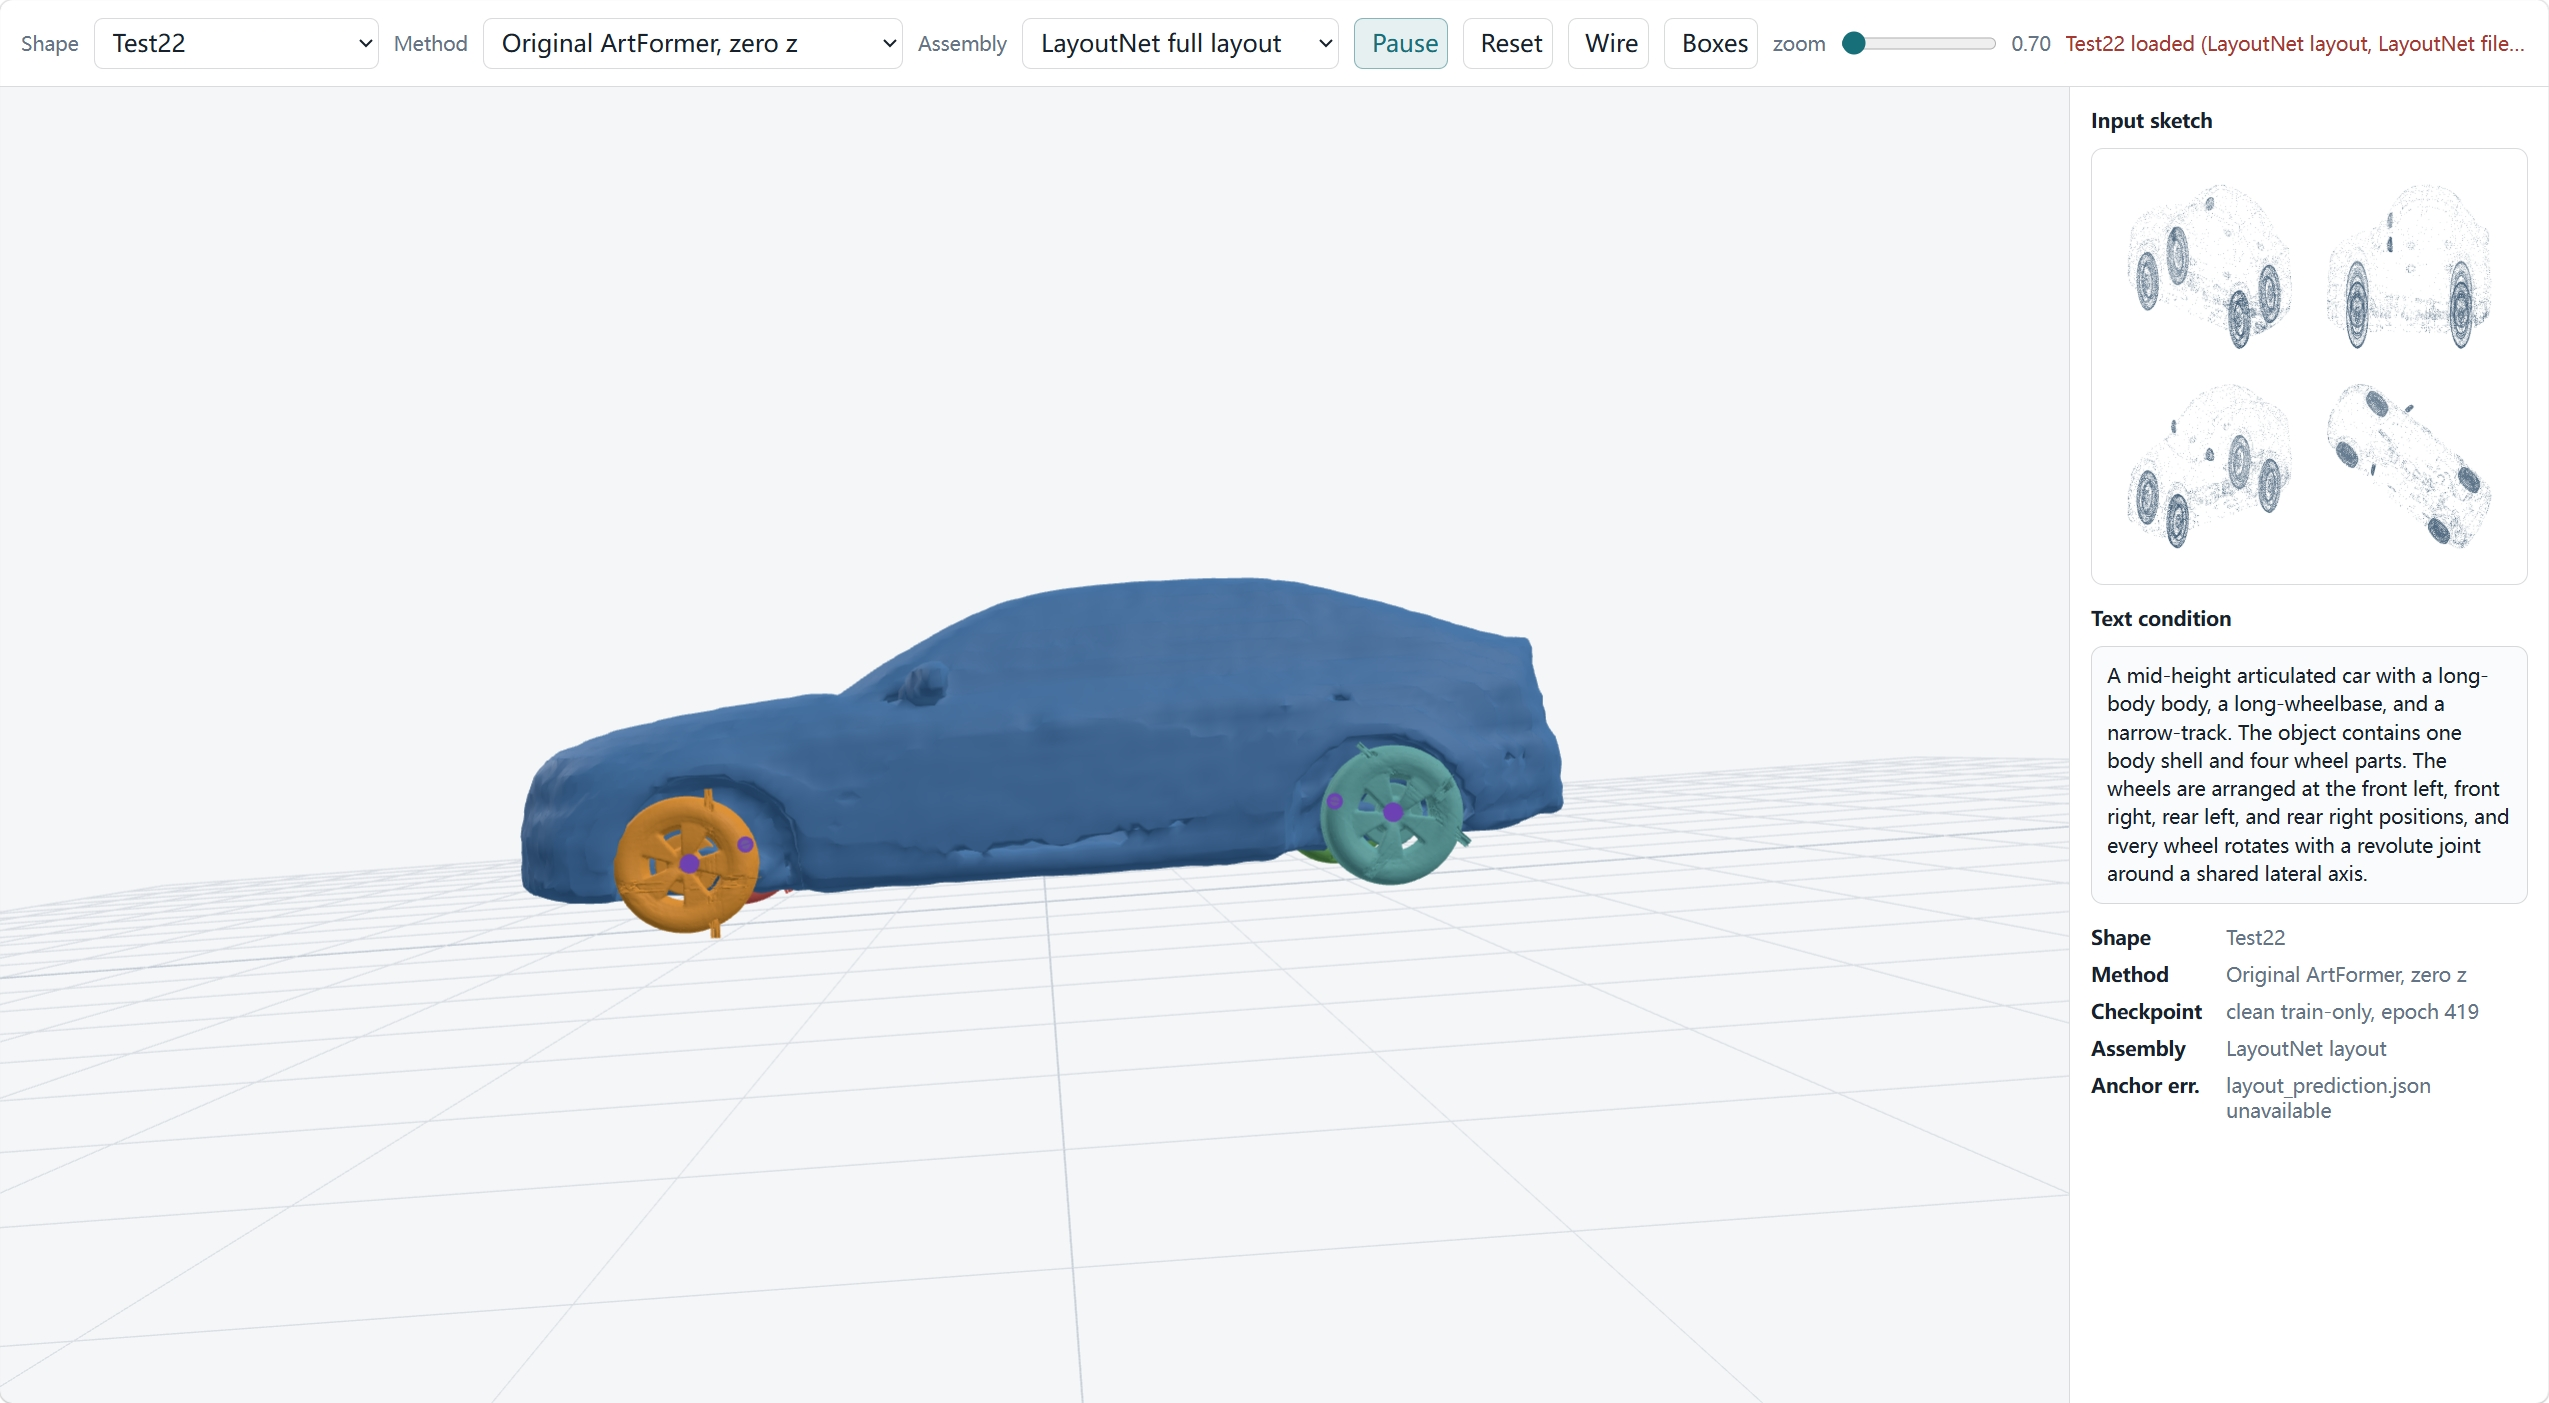
\includegraphics[width=0.30\linewidth]{ArtFormer_vs_CarActGen/ArtFormer_22.jpeg} &
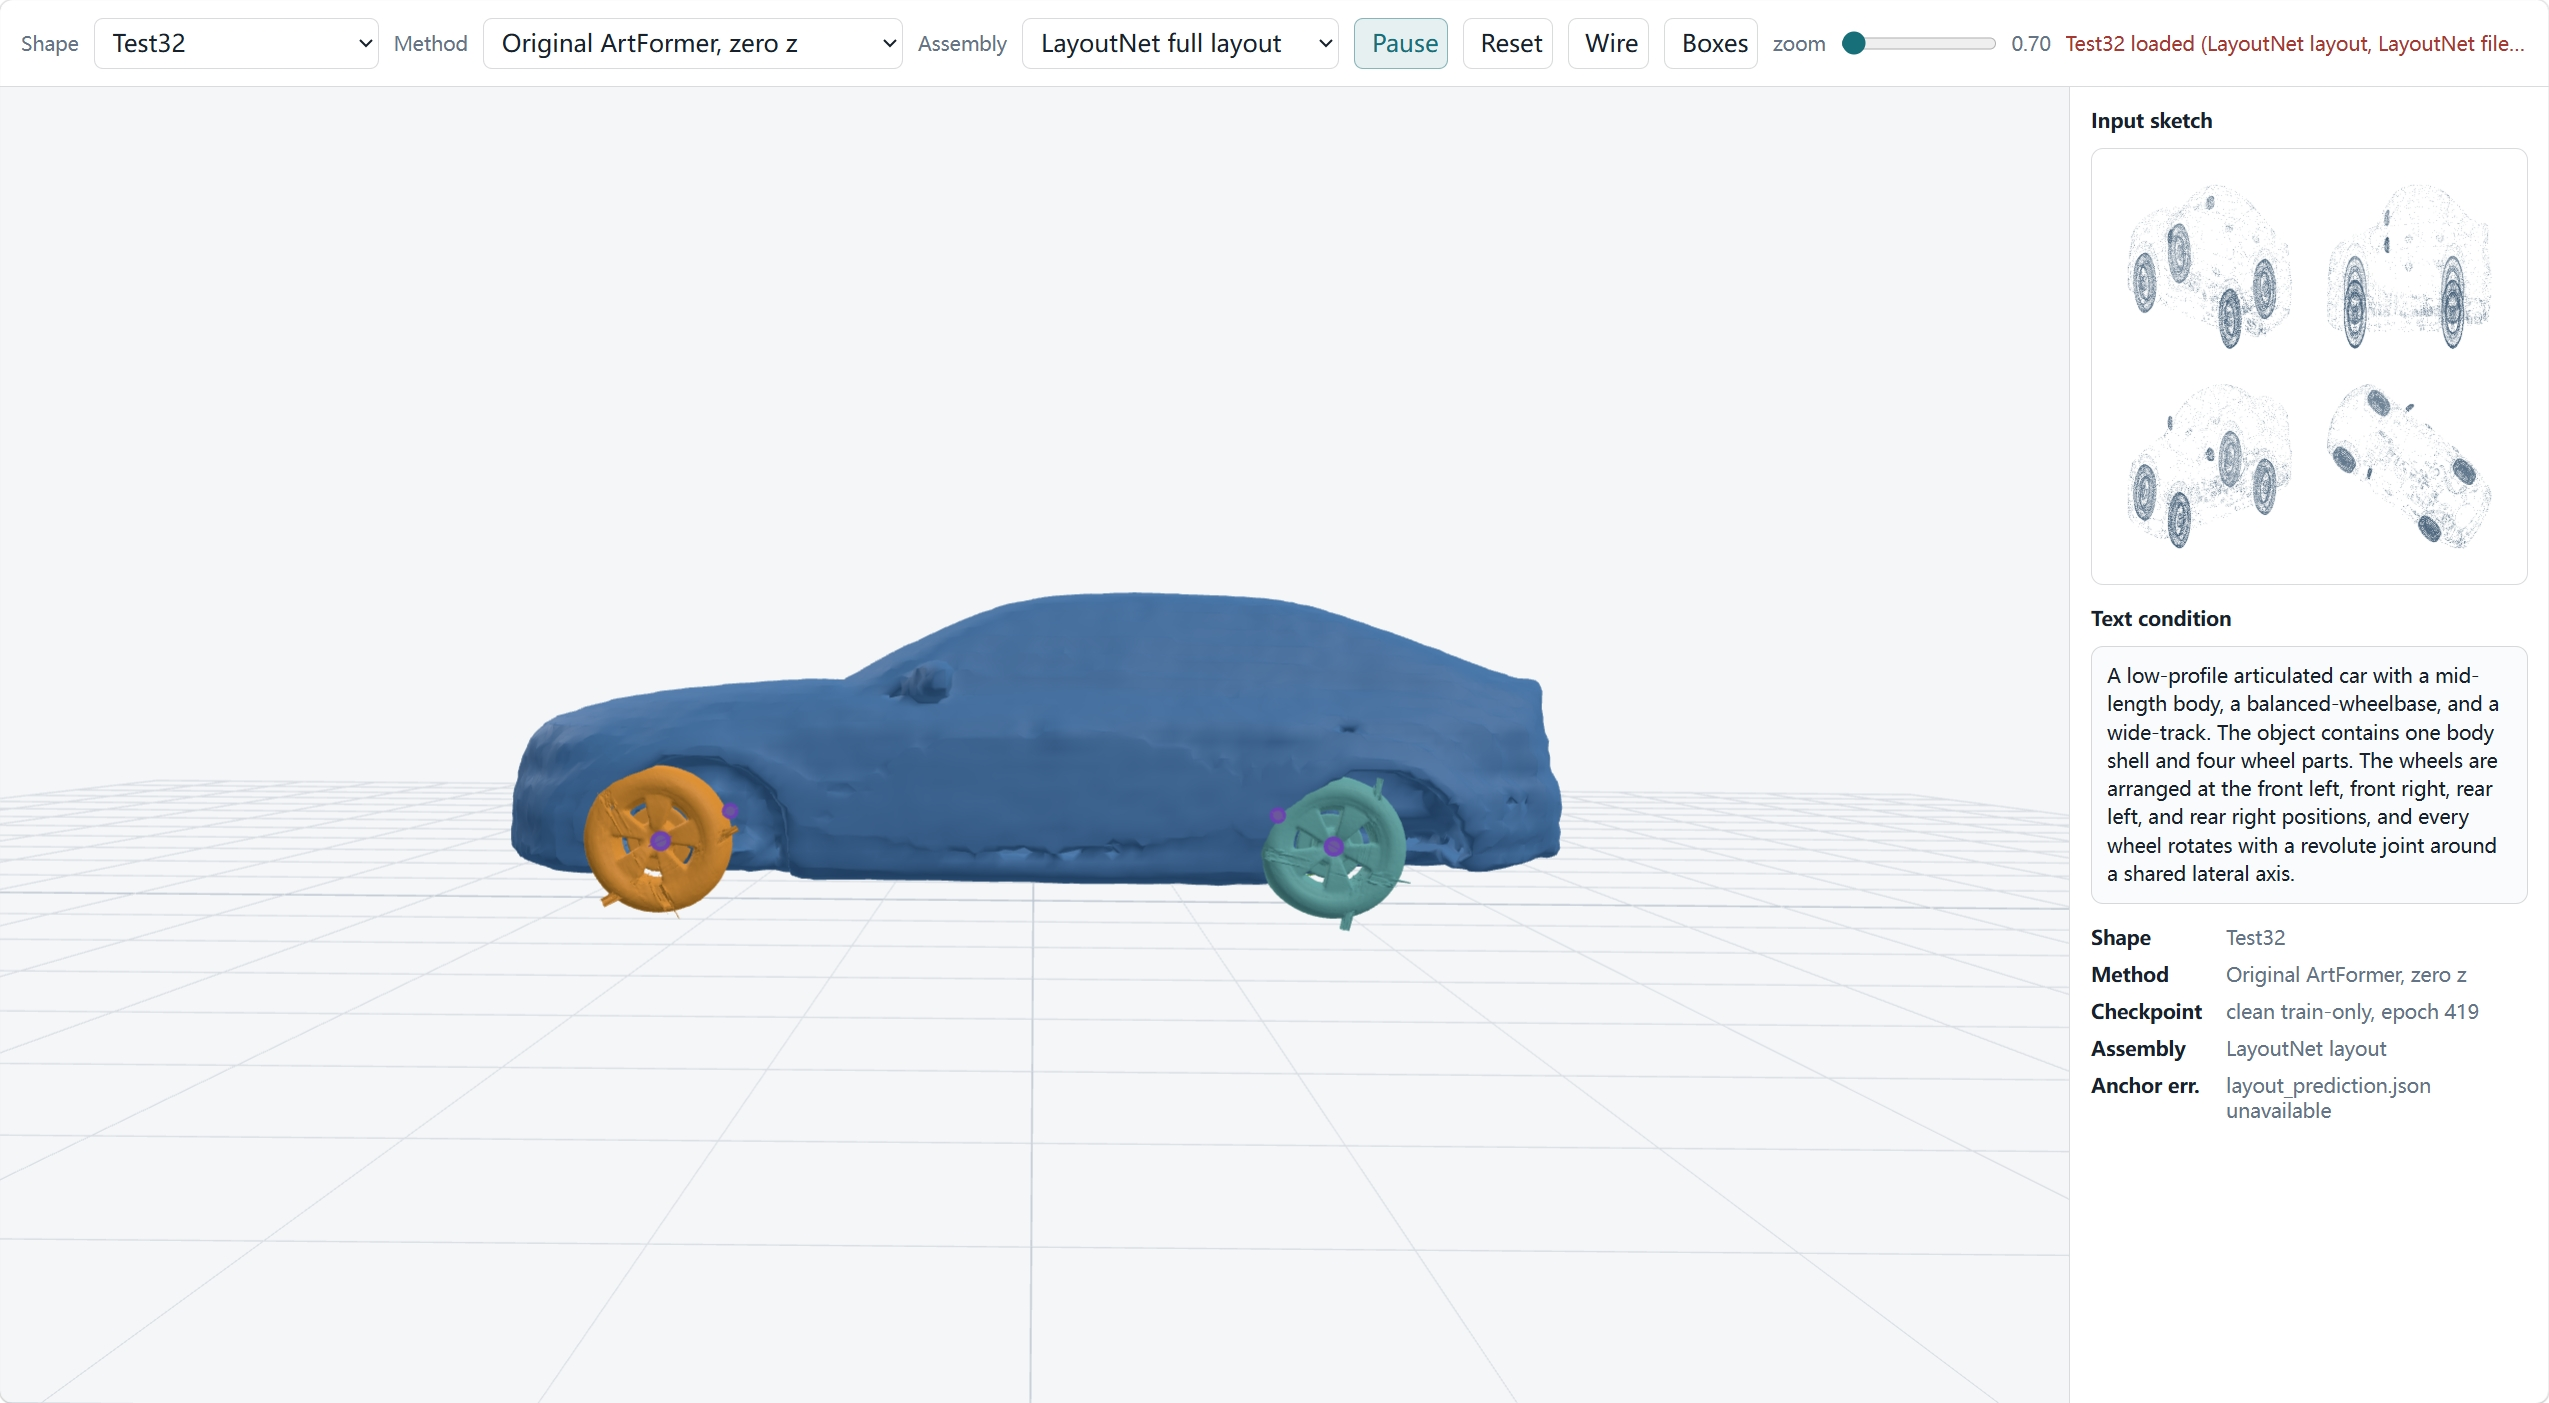
\includegraphics[width=0.30\linewidth]{ArtFormer_vs_CarActGen/ArtFormer_32.jpeg} &
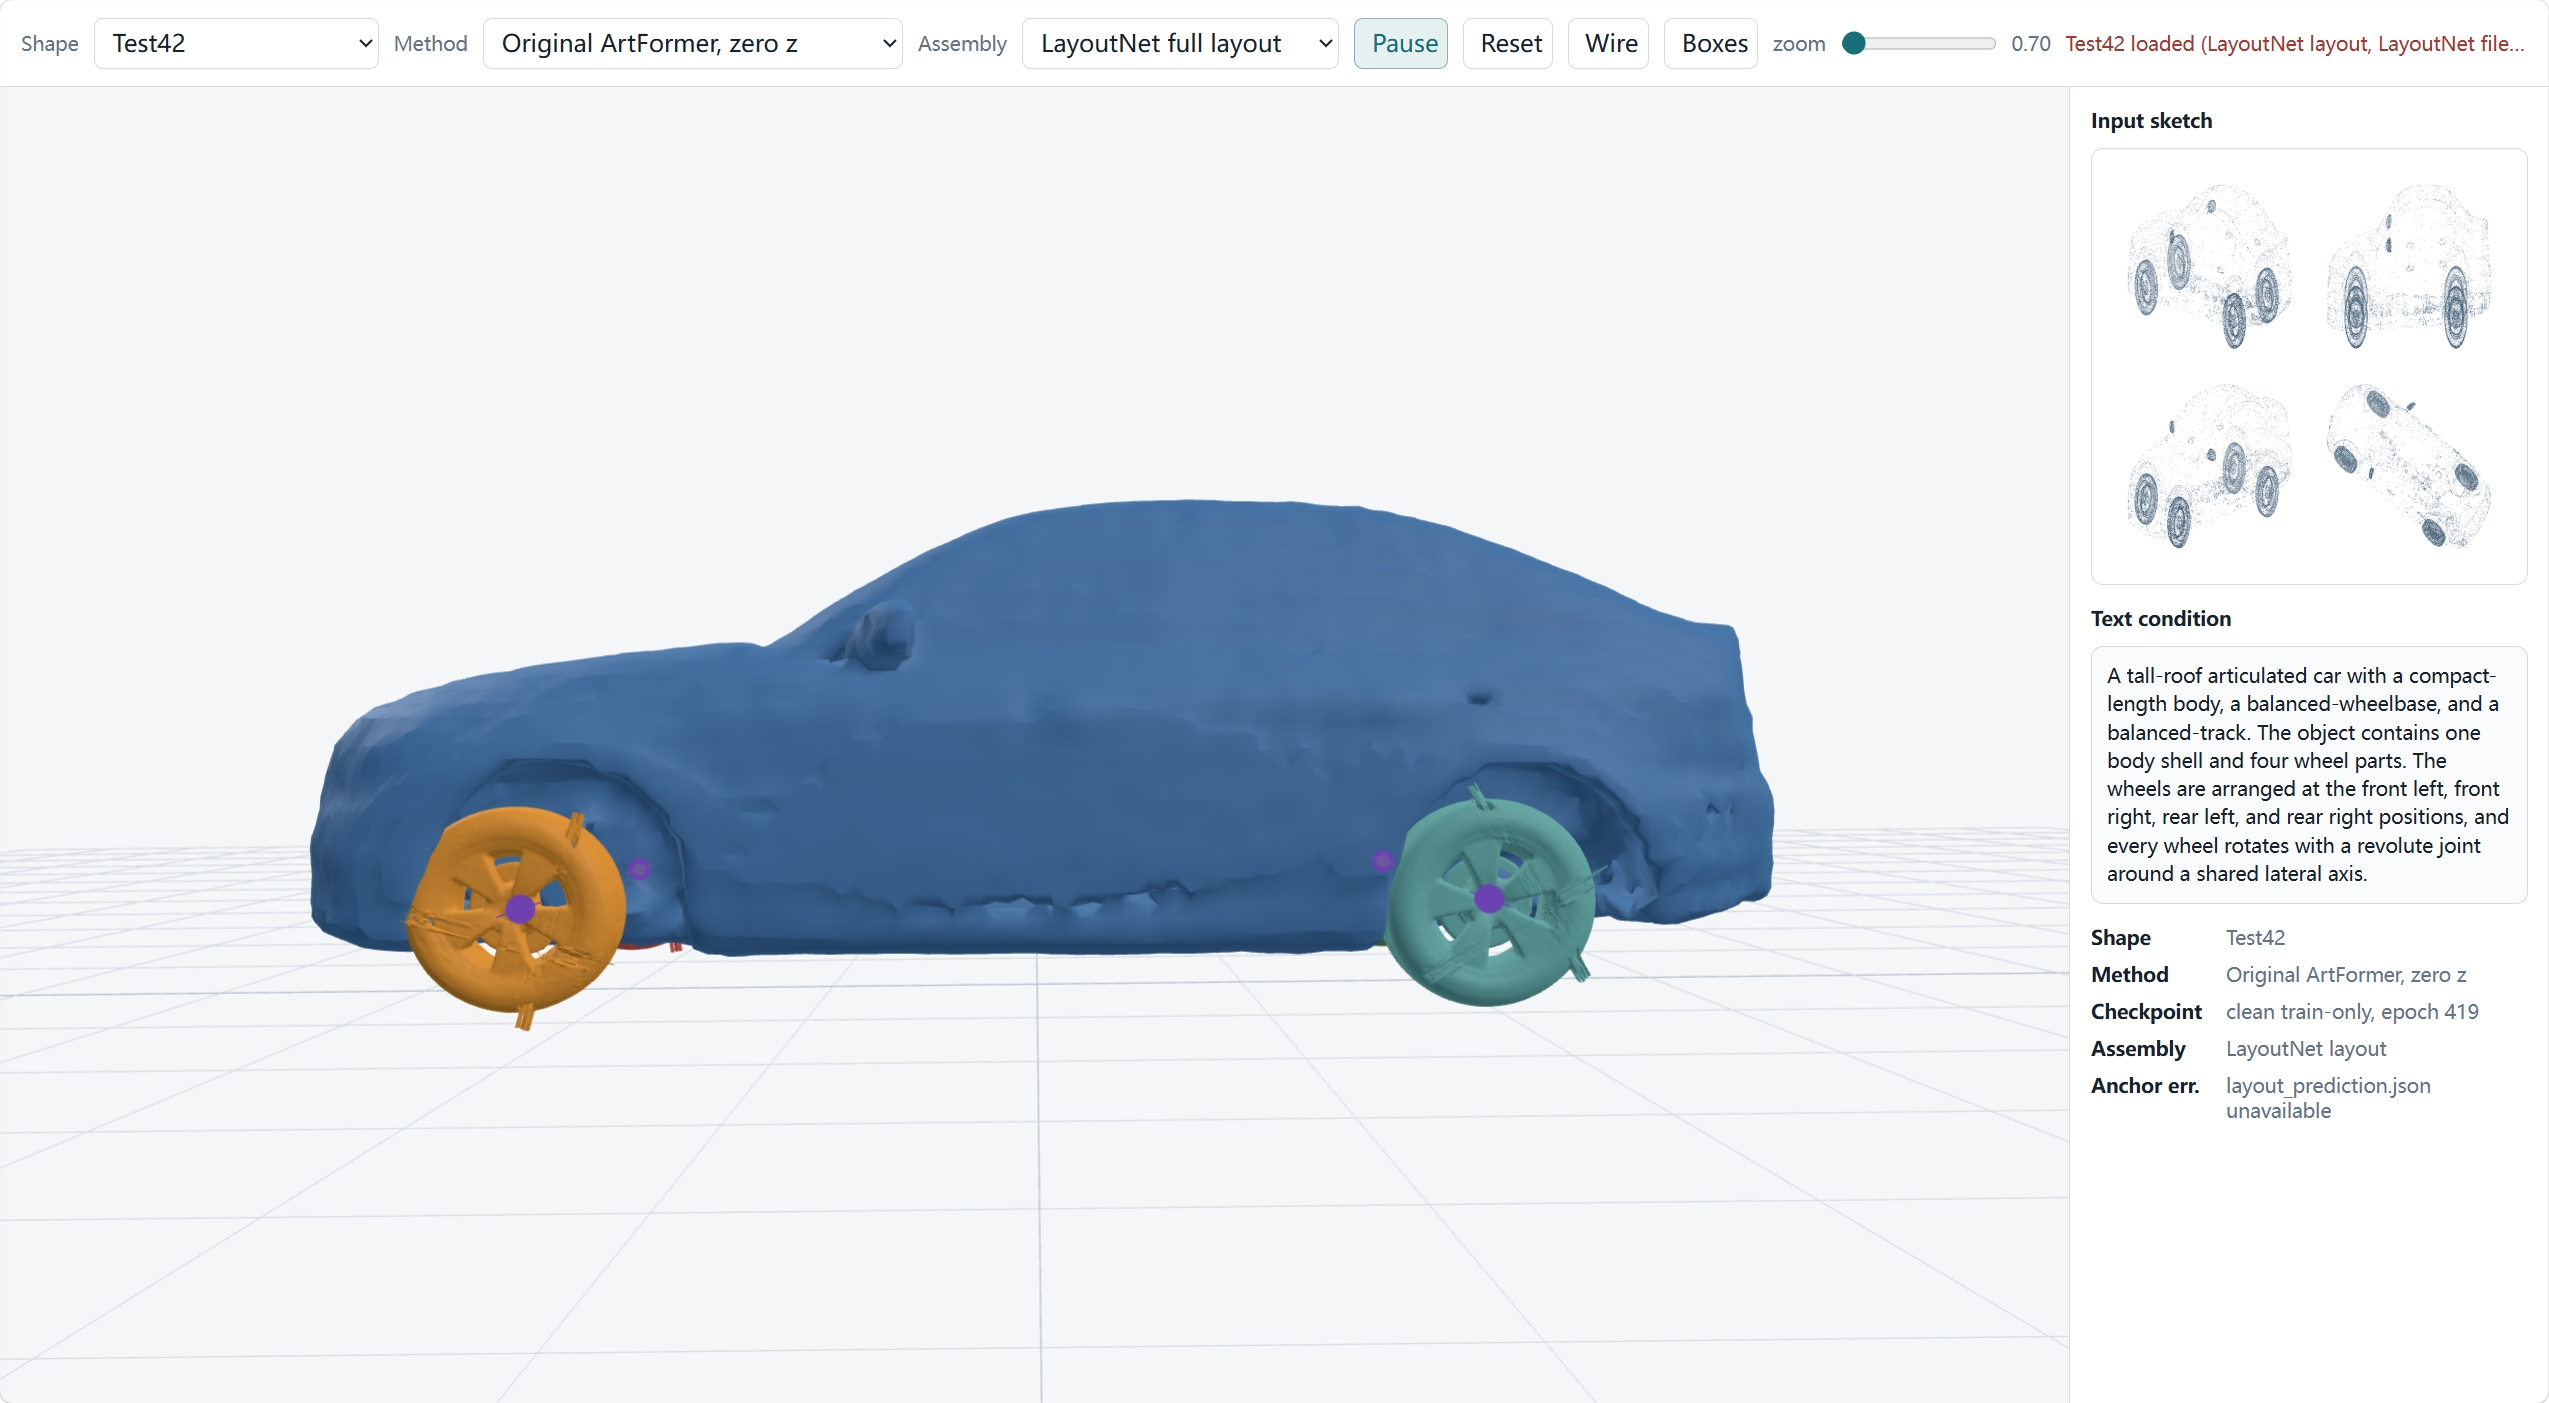
\includegraphics[width=0.30\linewidth]{ArtFormer_vs_CarActGen/ArtFormer_42.jpeg} \\
\small Original \artformer & \small Original \artformer & \small Original \artformer \\
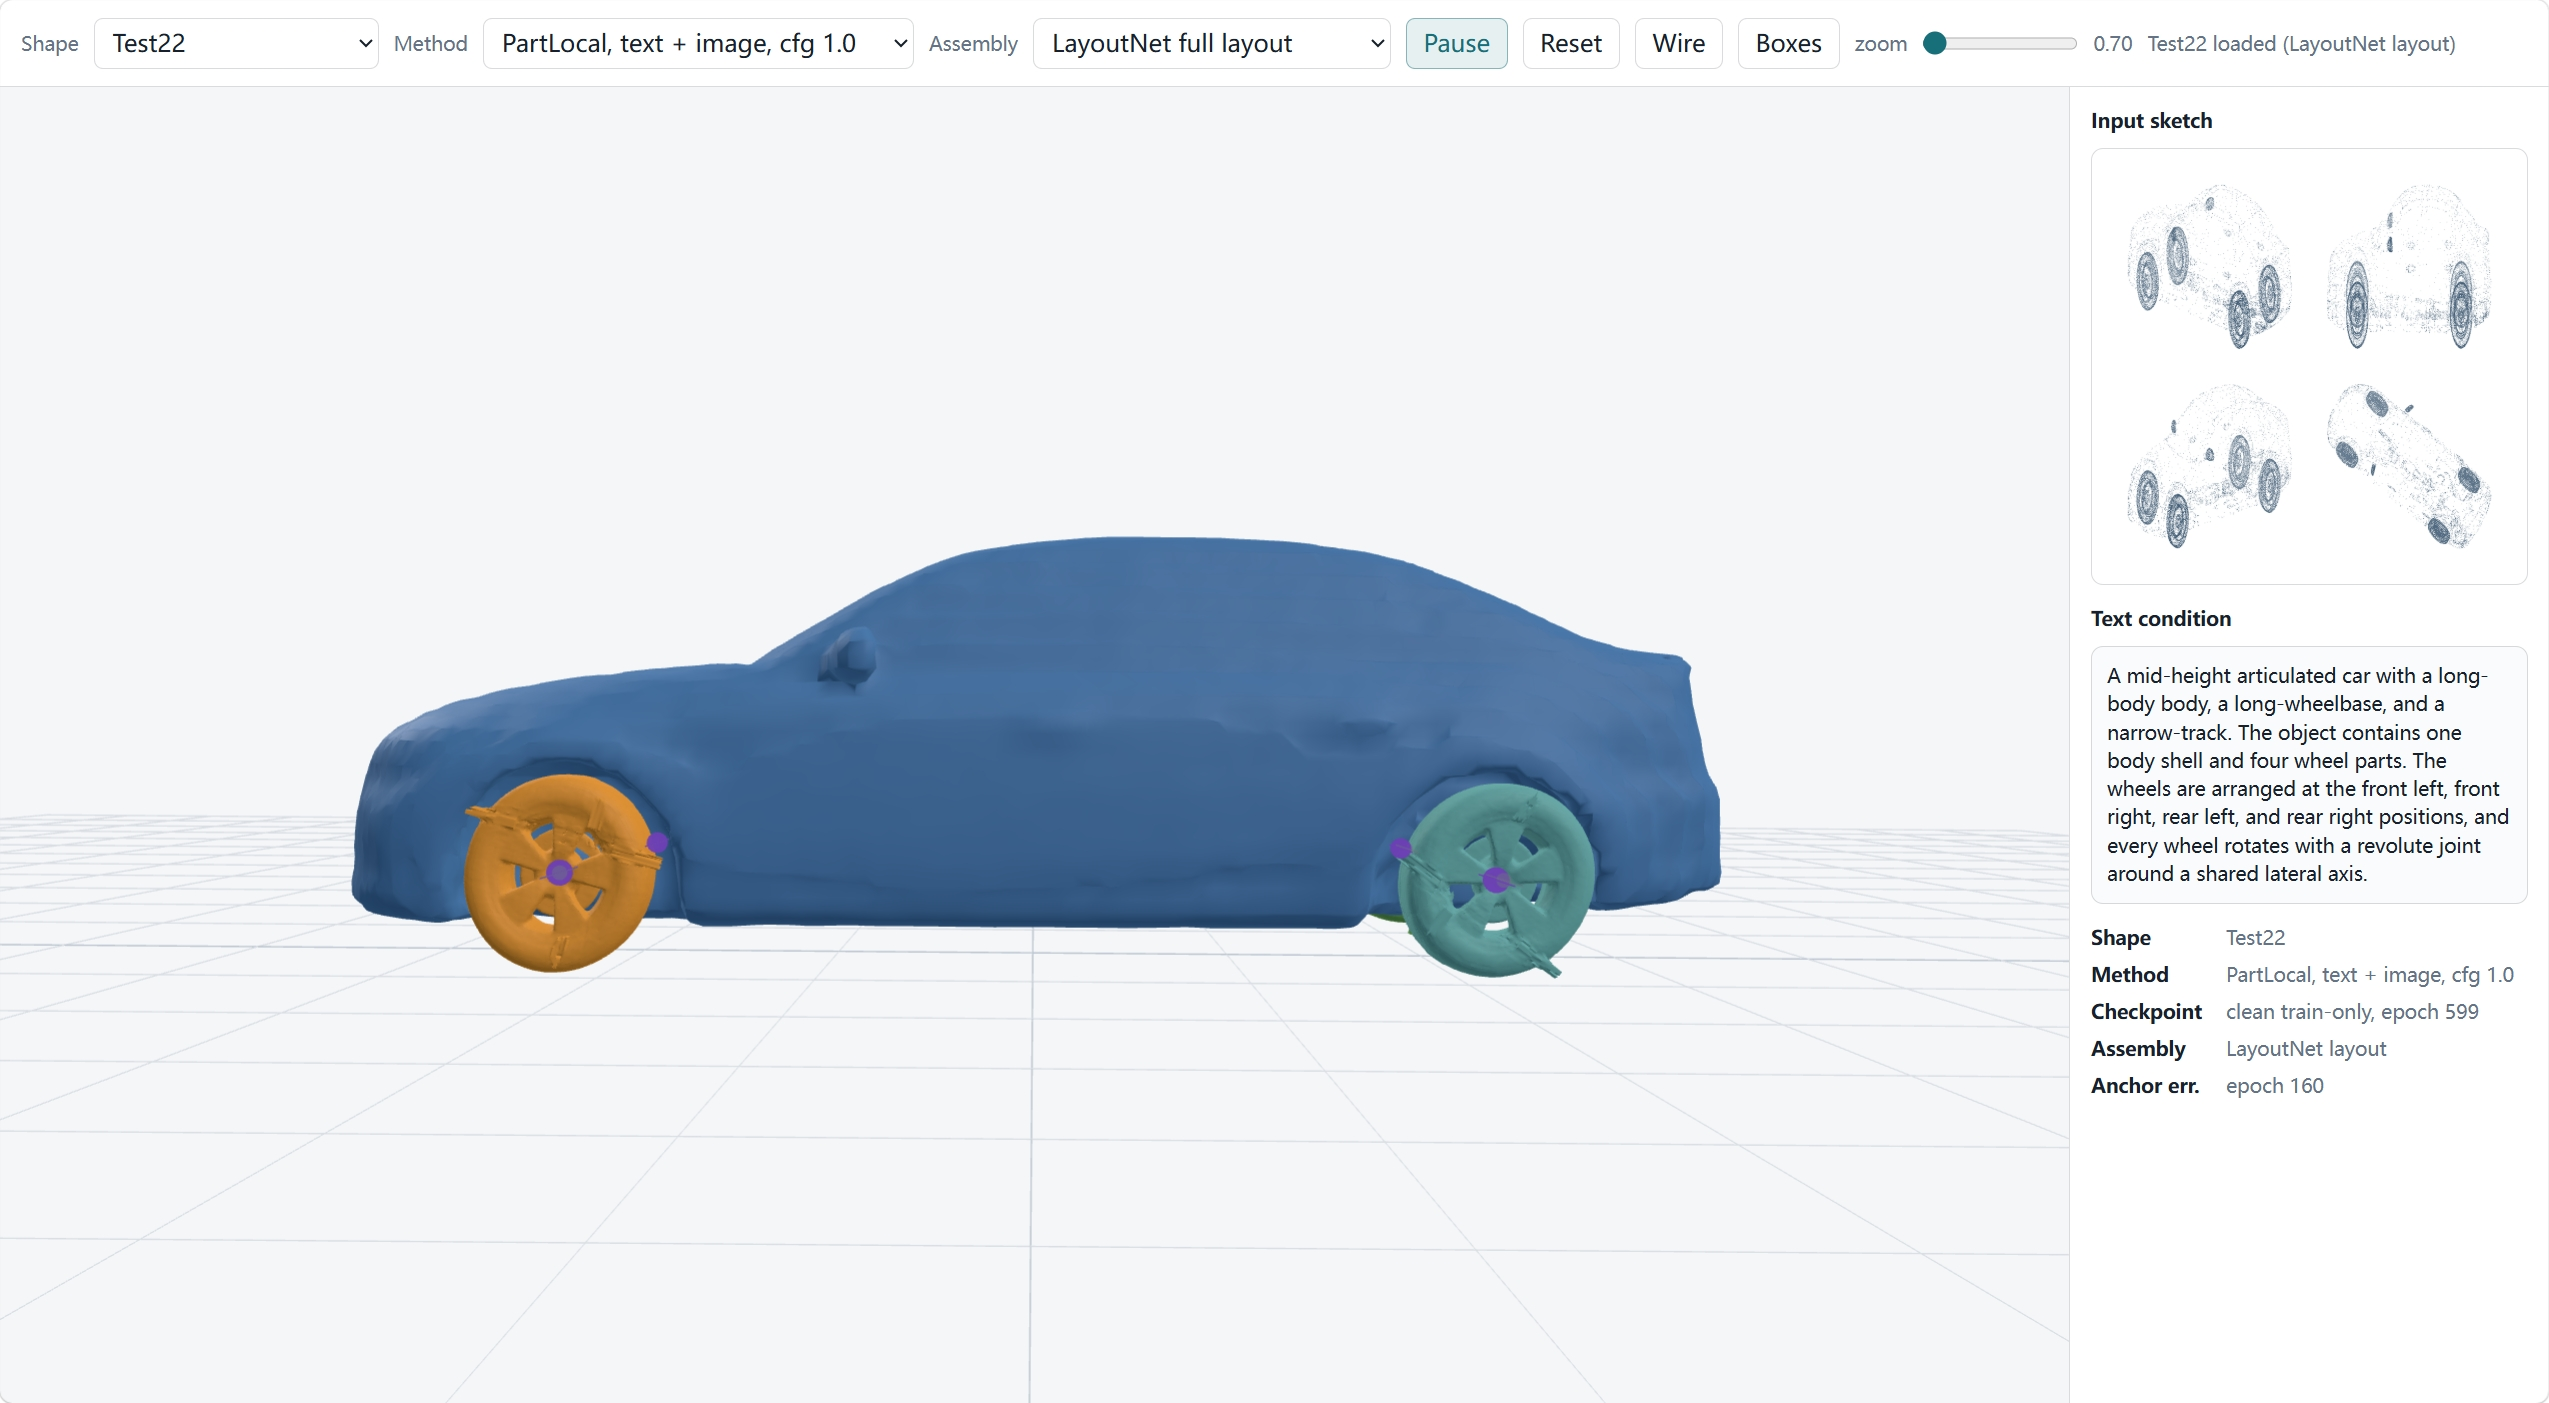
\includegraphics[width=0.30\linewidth]{ArtFormer_vs_CarActGen/CarActGen_22.jpeg} &
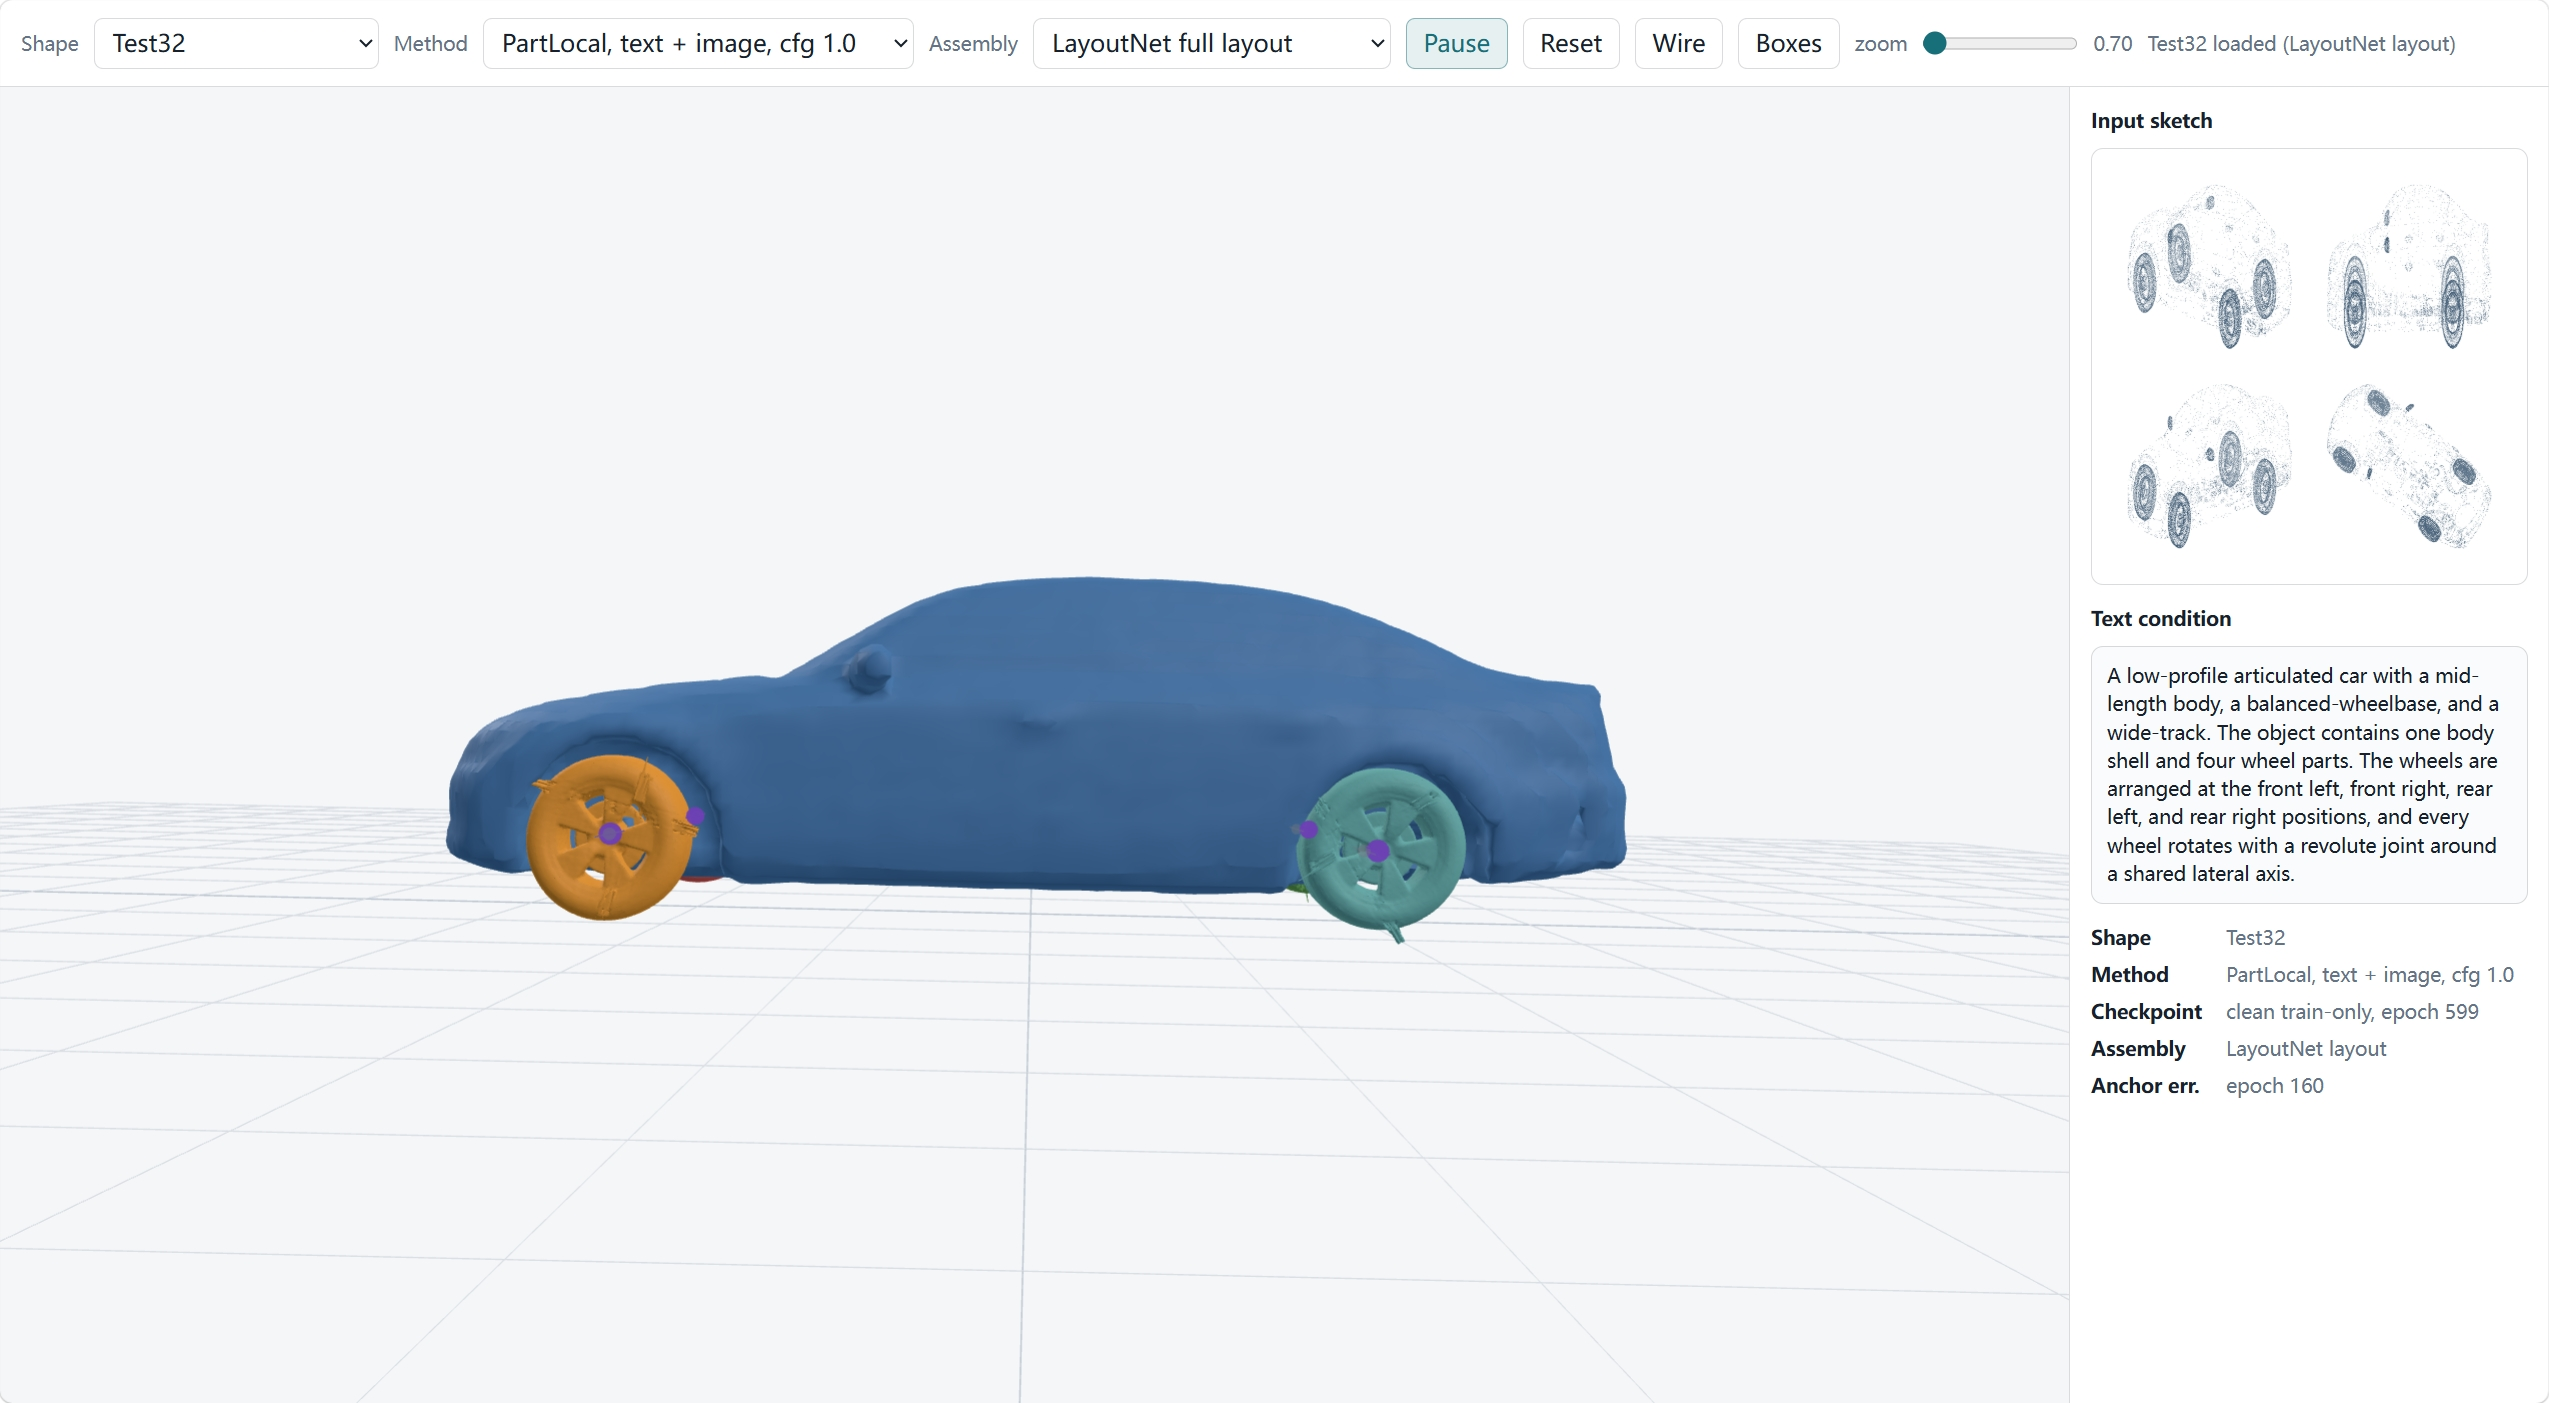
\includegraphics[width=0.30\linewidth]{ArtFormer_vs_CarActGen/CarActGen_32.jpeg} &
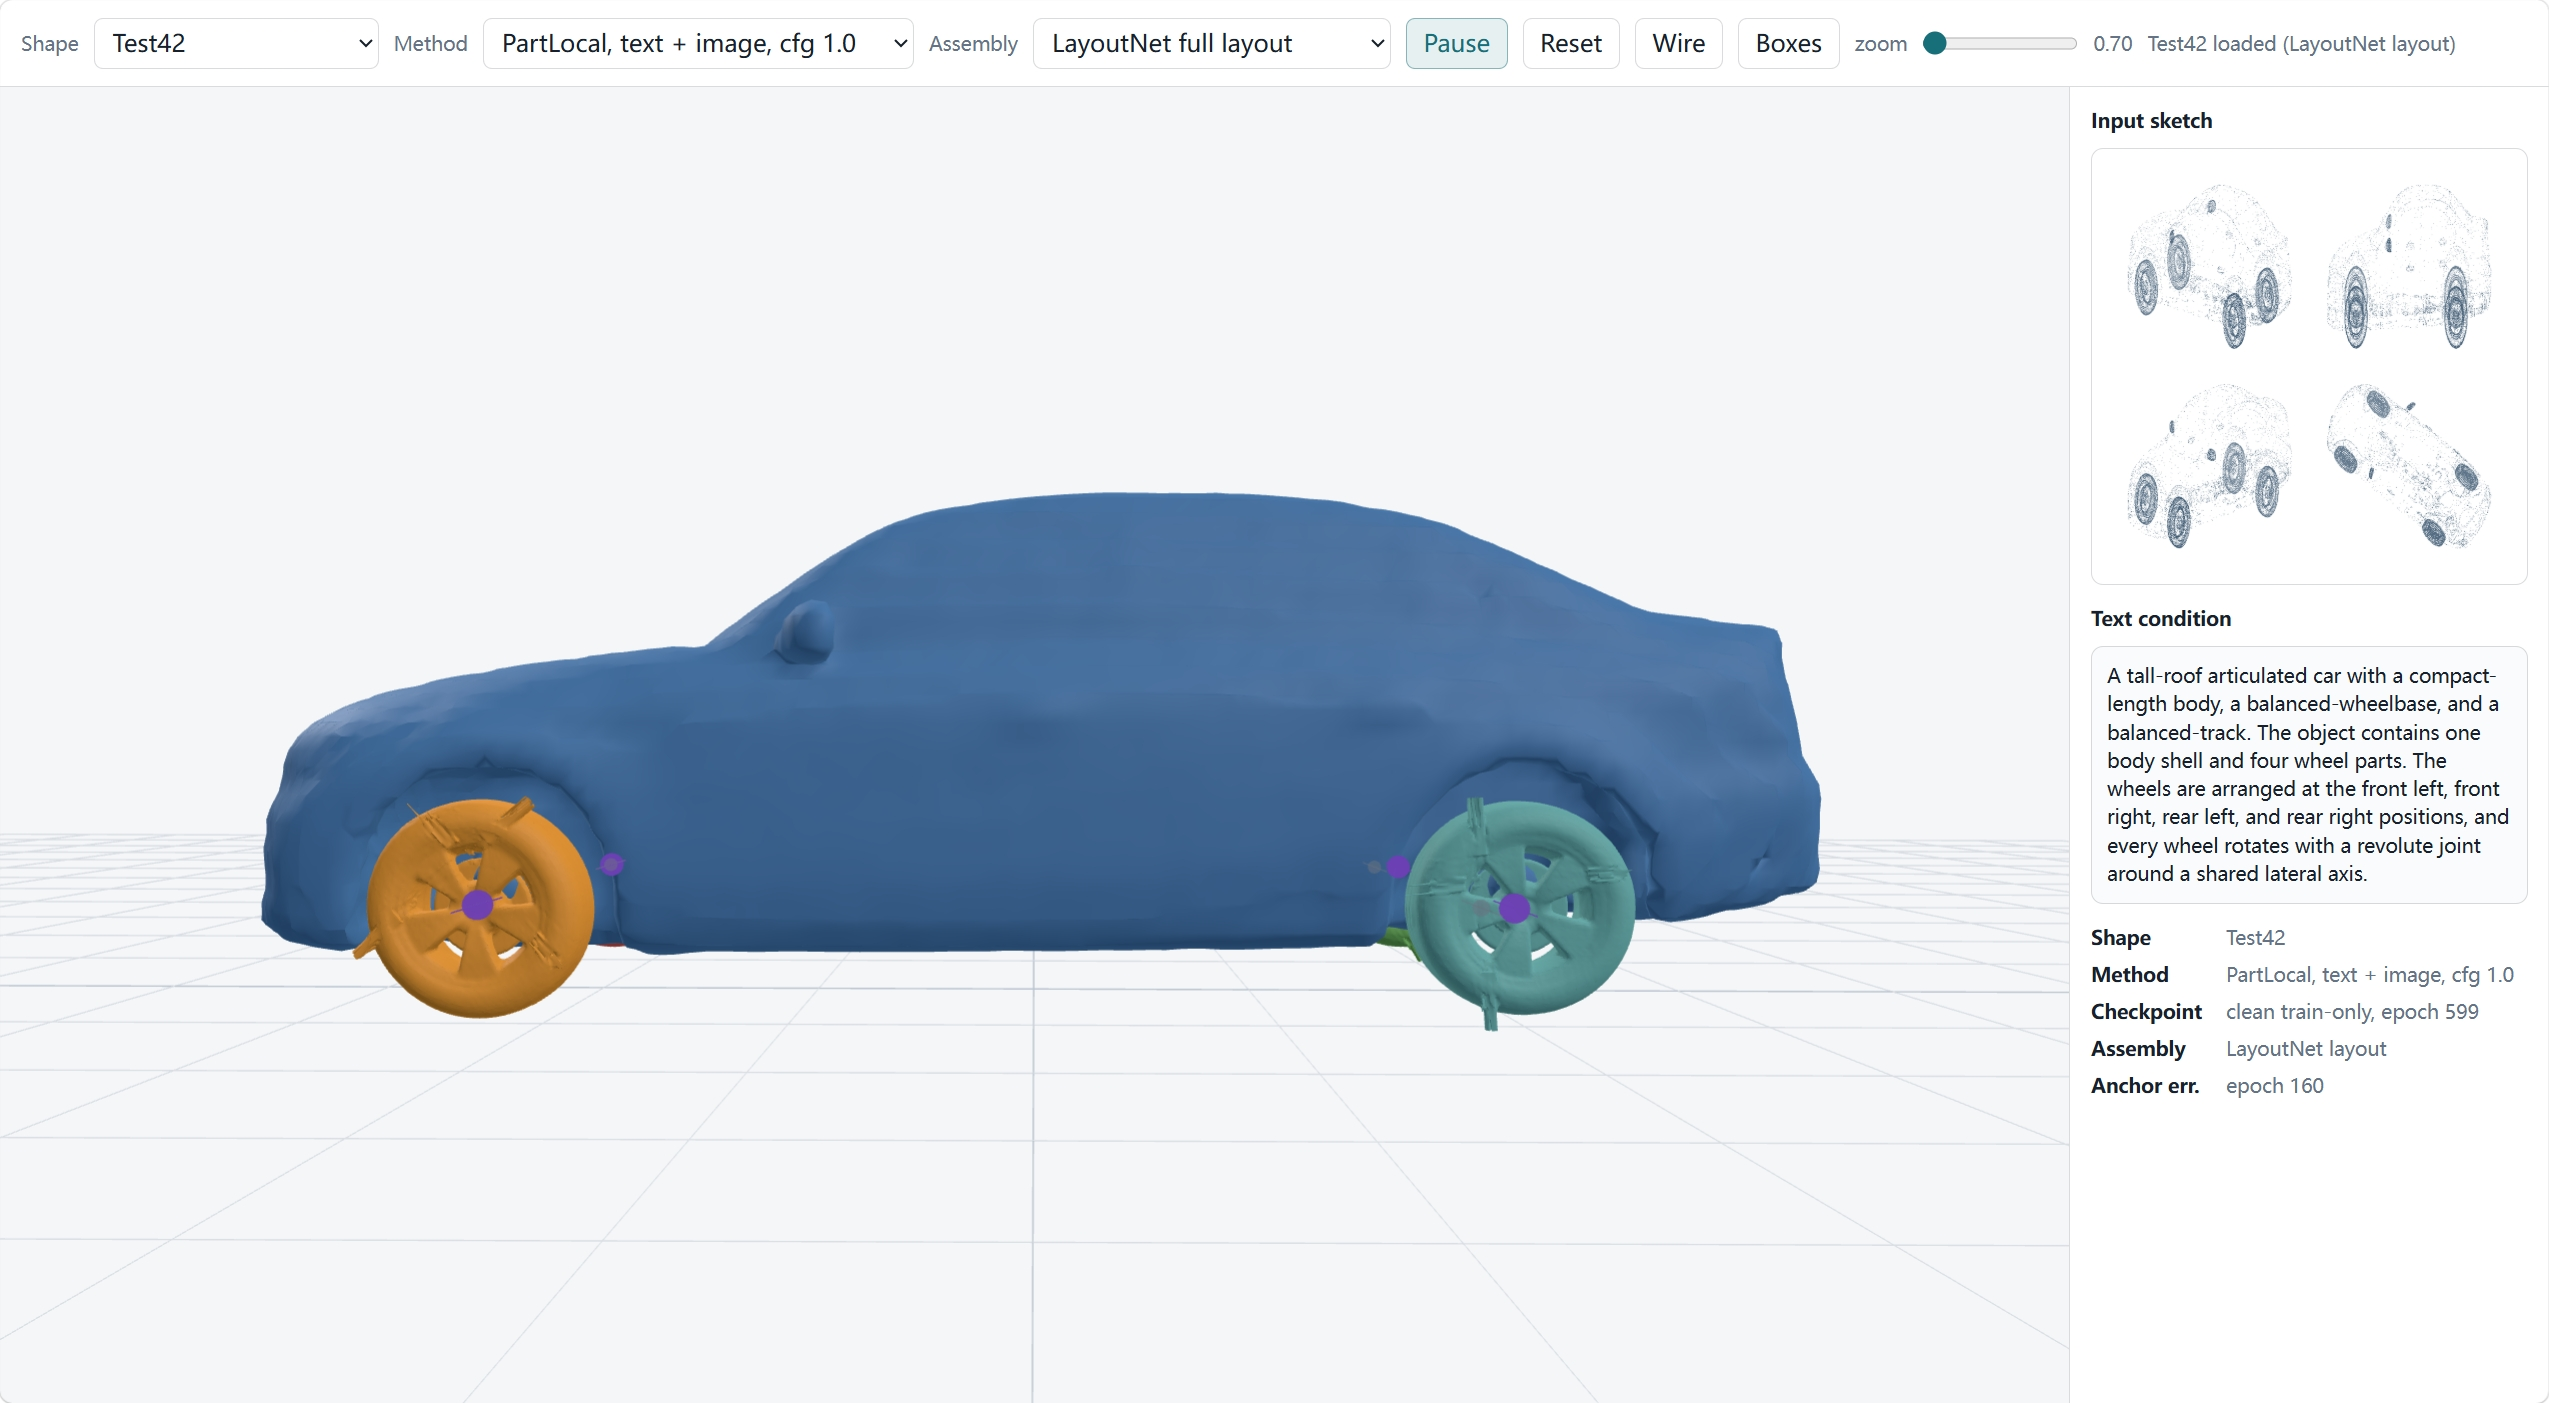
\includegraphics[width=0.30\linewidth]{ArtFormer_vs_CarActGen/CarActGen_42.jpeg} \\
\small \method & \small \method & \small \method
\end{tabular}
\caption{Qualitative comparison between the original \artformer baseline and \method. The \method body surfaces are smoother and contain fewer local artifacts, while wheel differences are less salient because wheels cover a smaller visual area.}
\label{fig:qualitative-grid}
\end{figure}

Figure~\ref{fig:condition-comparison} compares different conditioning modes. The fused text+sketch condition gives the best geometry quality in this example. At the same time, text-only conditioning shows slightly stronger control over the generated shape, while sketch-only conditioning is weaker and depends heavily on a DrivAer-style sketch input. This limitation is likely caused by the dataset: both training and evaluation sketches come from a narrow DrivAerML-style rendering process, so the sketch branch has limited evidence for out-of-domain hand-drawn inputs.

\begin{figure}[t]
\centering
\begin{tabular}{@{}ccc@{}}
\textbf{Text} & \textbf{Sketch} & \textbf{Text+Sketch} \\
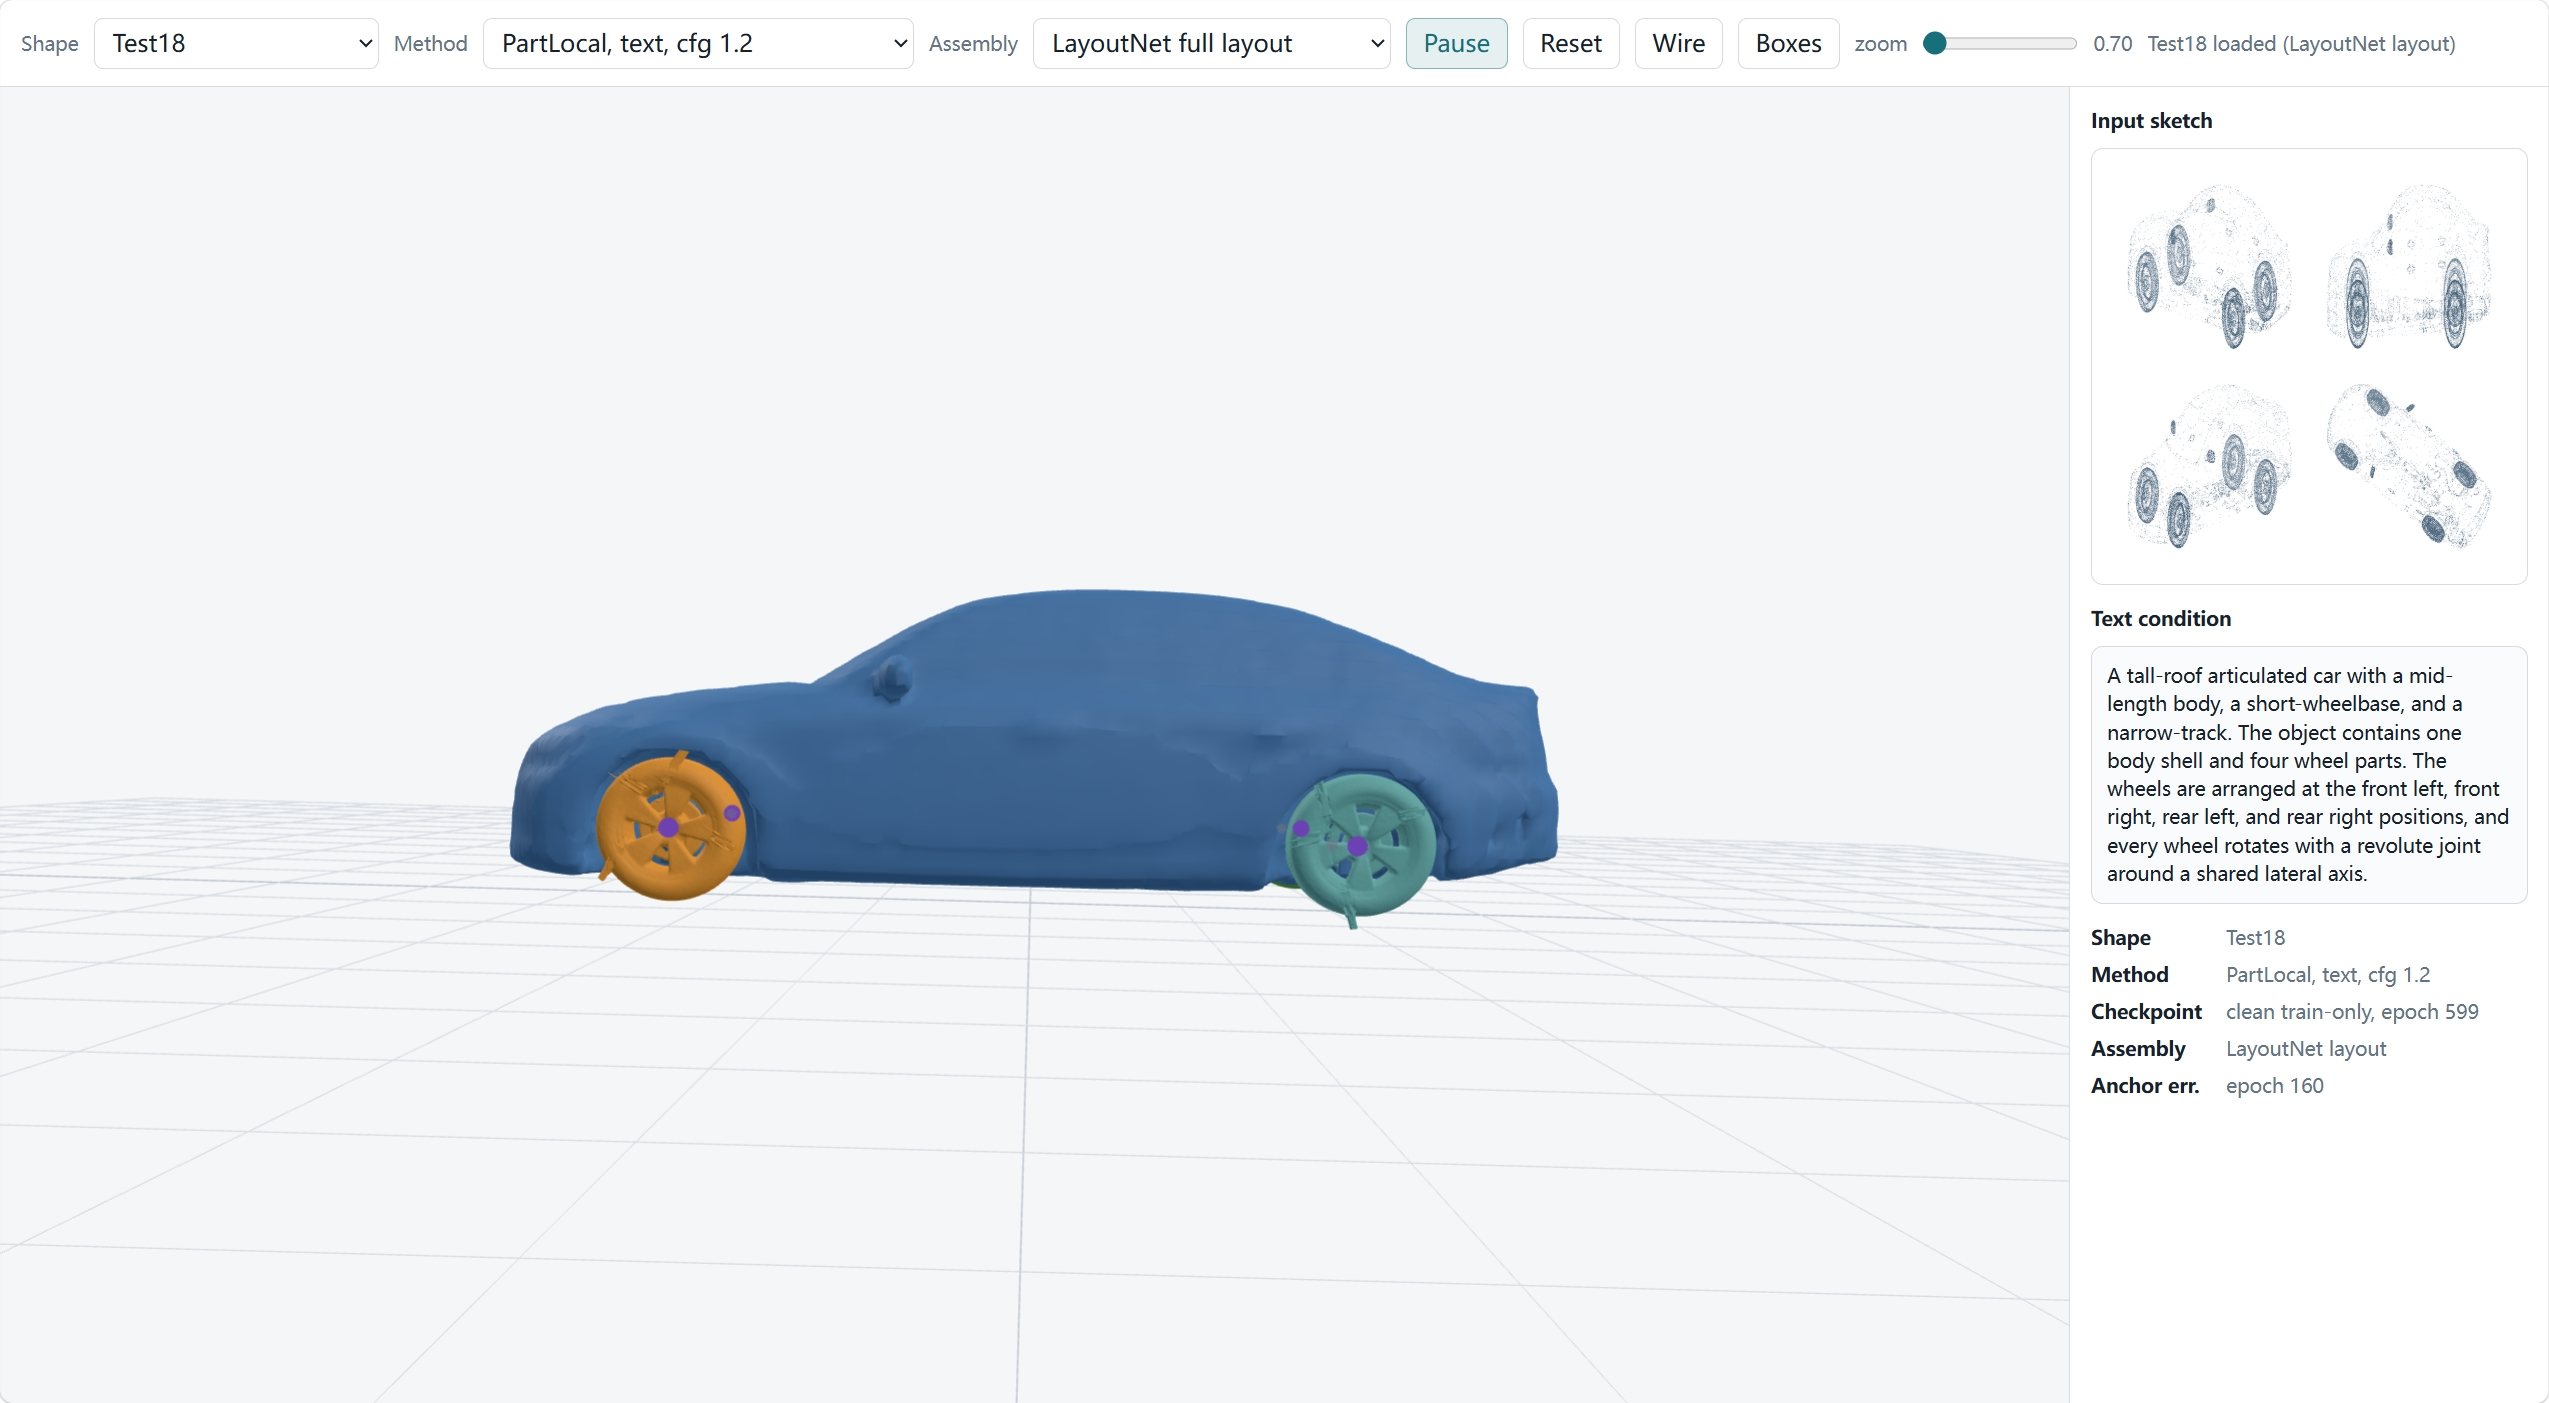
\includegraphics[width=0.30\linewidth]{Text_vs_Image/Text_18.jpeg} &
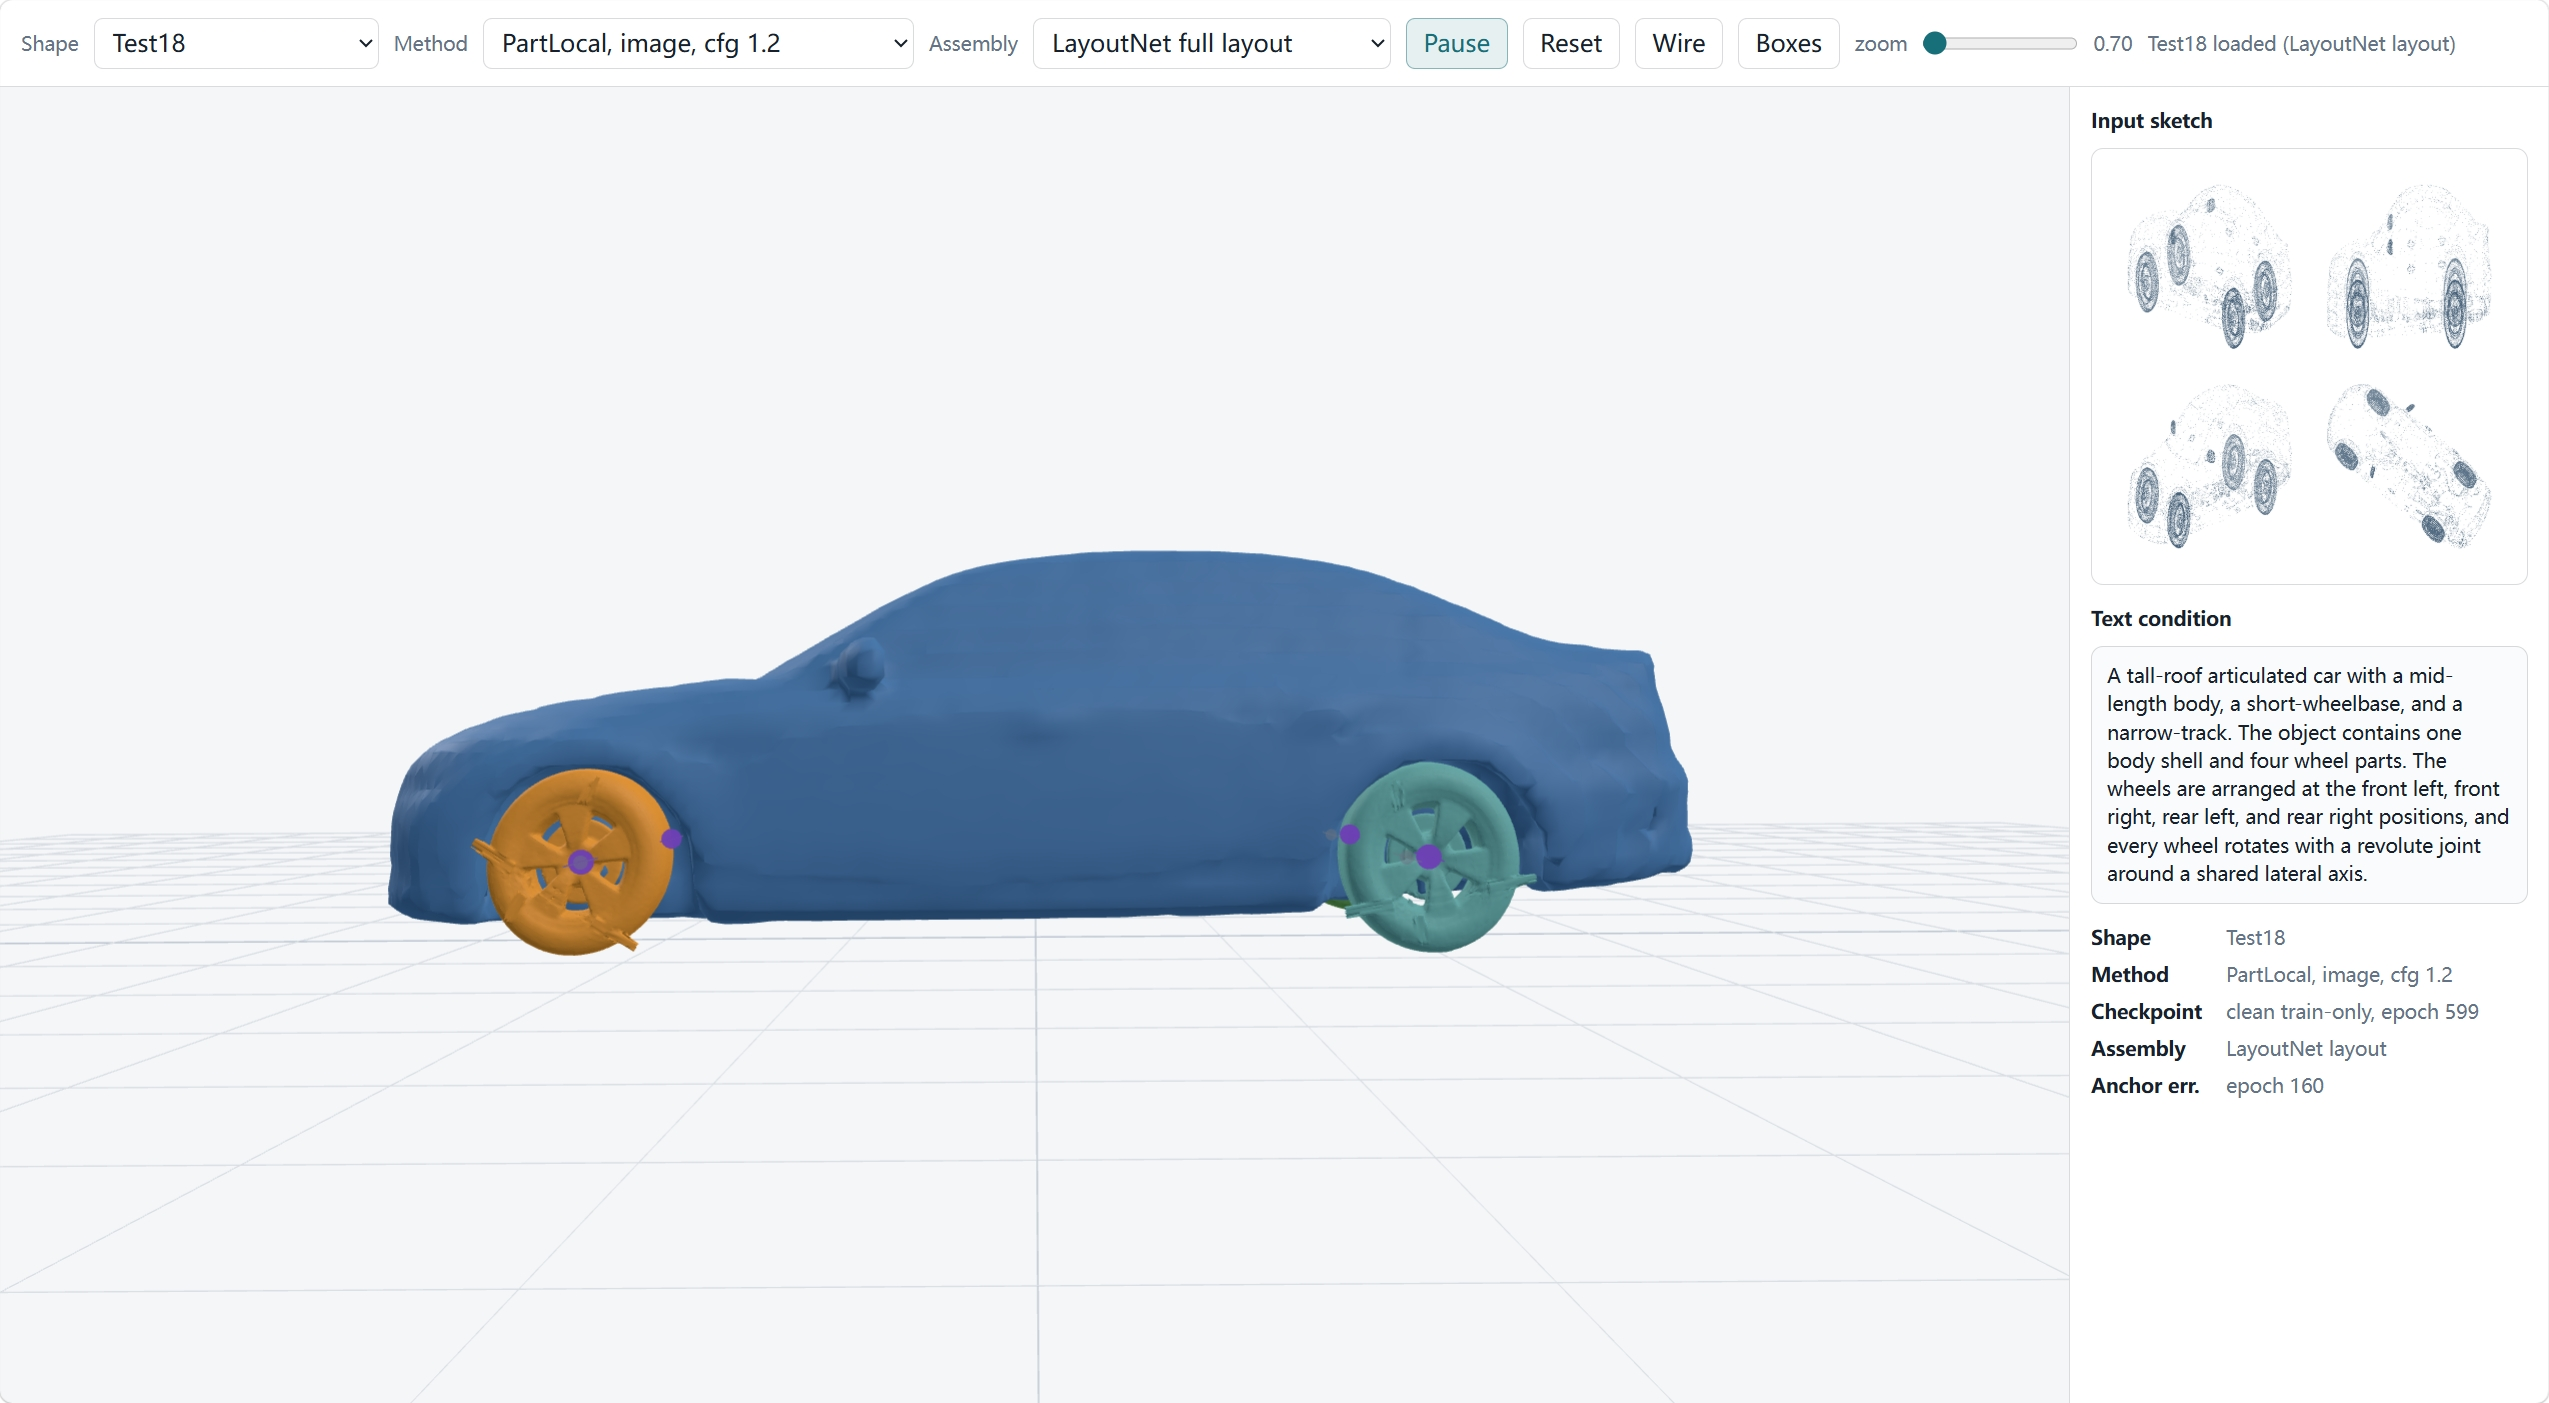
\includegraphics[width=0.30\linewidth]{Text_vs_Image/image_18.jpeg} &
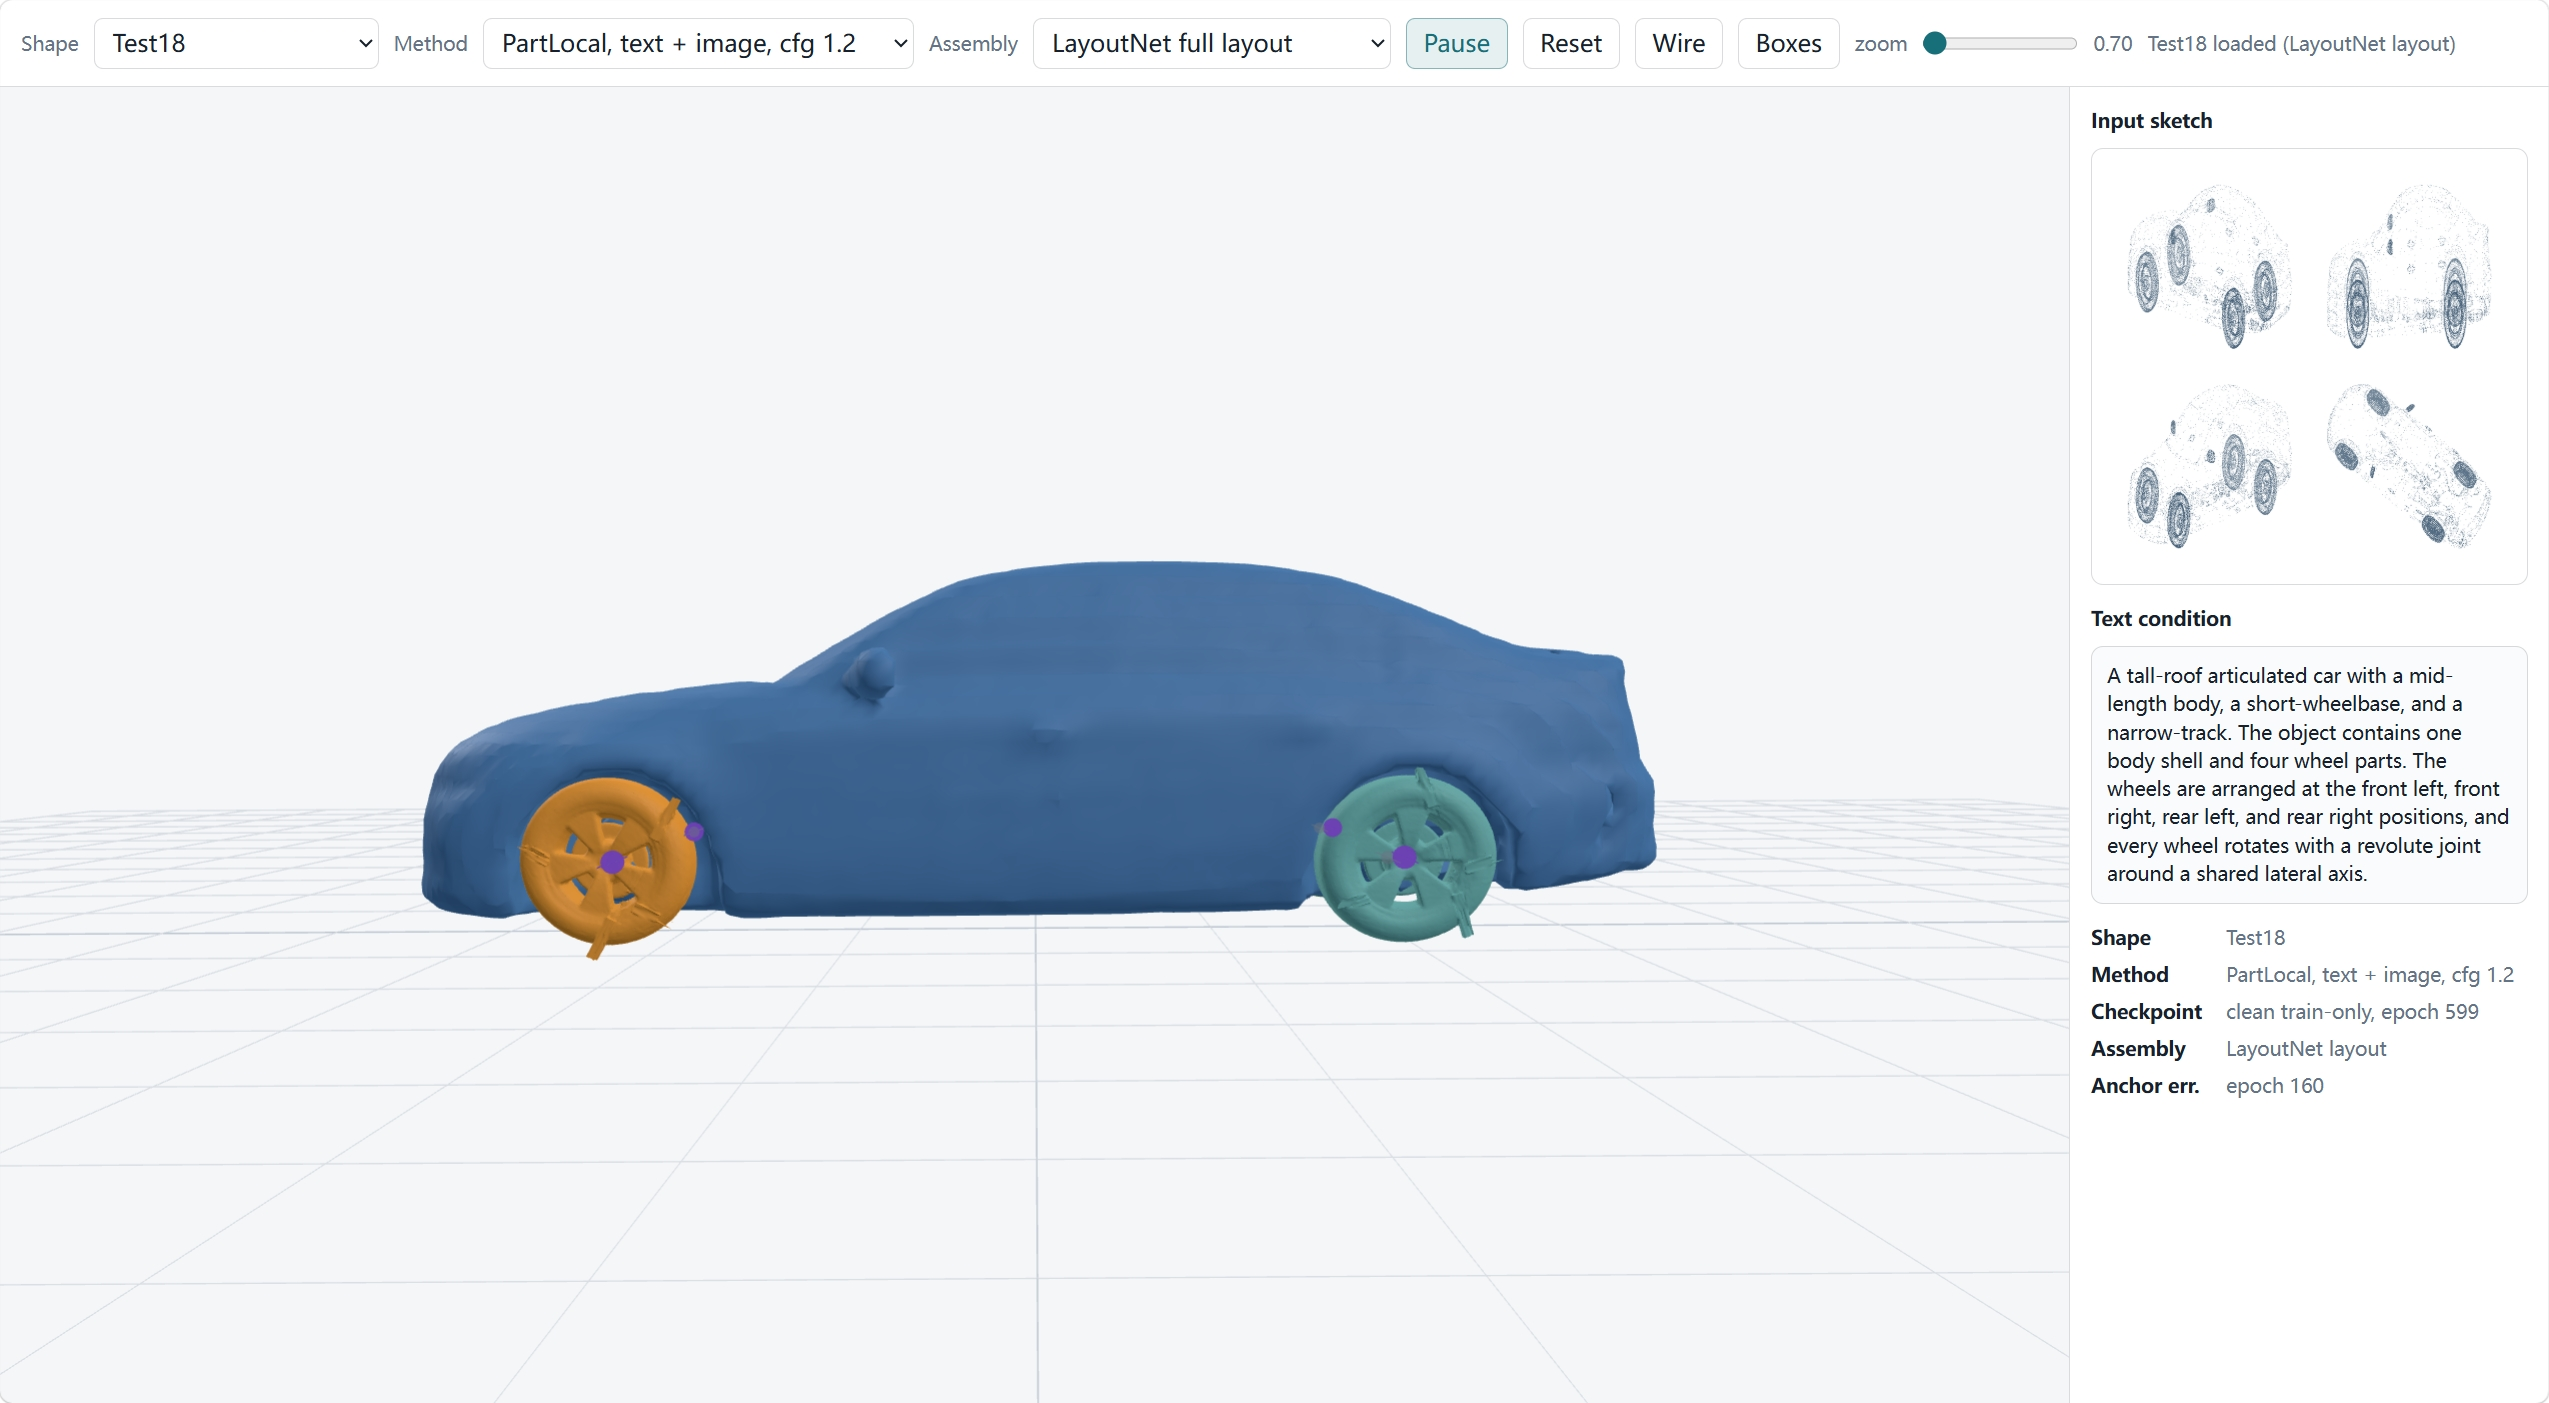
\includegraphics[width=0.30\linewidth]{Text_vs_Image/Text+Image_18.jpeg}
\end{tabular}
\caption{Comparison of text, sketch, and fused text+sketch conditioning. Text gives more direct semantic control over coarse shape, while sketch conditioning is useful but currently tied to DrivAer-style inputs.}
\label{fig:condition-comparison}
\end{figure}

Finally, Figure~\ref{fig:layout-comparison} compares two end-to-end assembly modes that do not require a concrete source bounding box at test time. The ClassMean layout uses a fixed train-set mean template, while LayoutNet predicts boxes and wheel pivots from the generated representation and conditions. ClassMean often produces off-center wheel axes, which appears as eccentric tire rotation in the viewer. LayoutNet places the joints much closer to the wheel centers, confirming that learnable layout prediction is an effective design for functional assembly.

\begin{figure}[t]
\centering
\begin{tabular}{@{}cc@{}}
\textbf{ClassMean} & \textbf{LayoutNet} \\
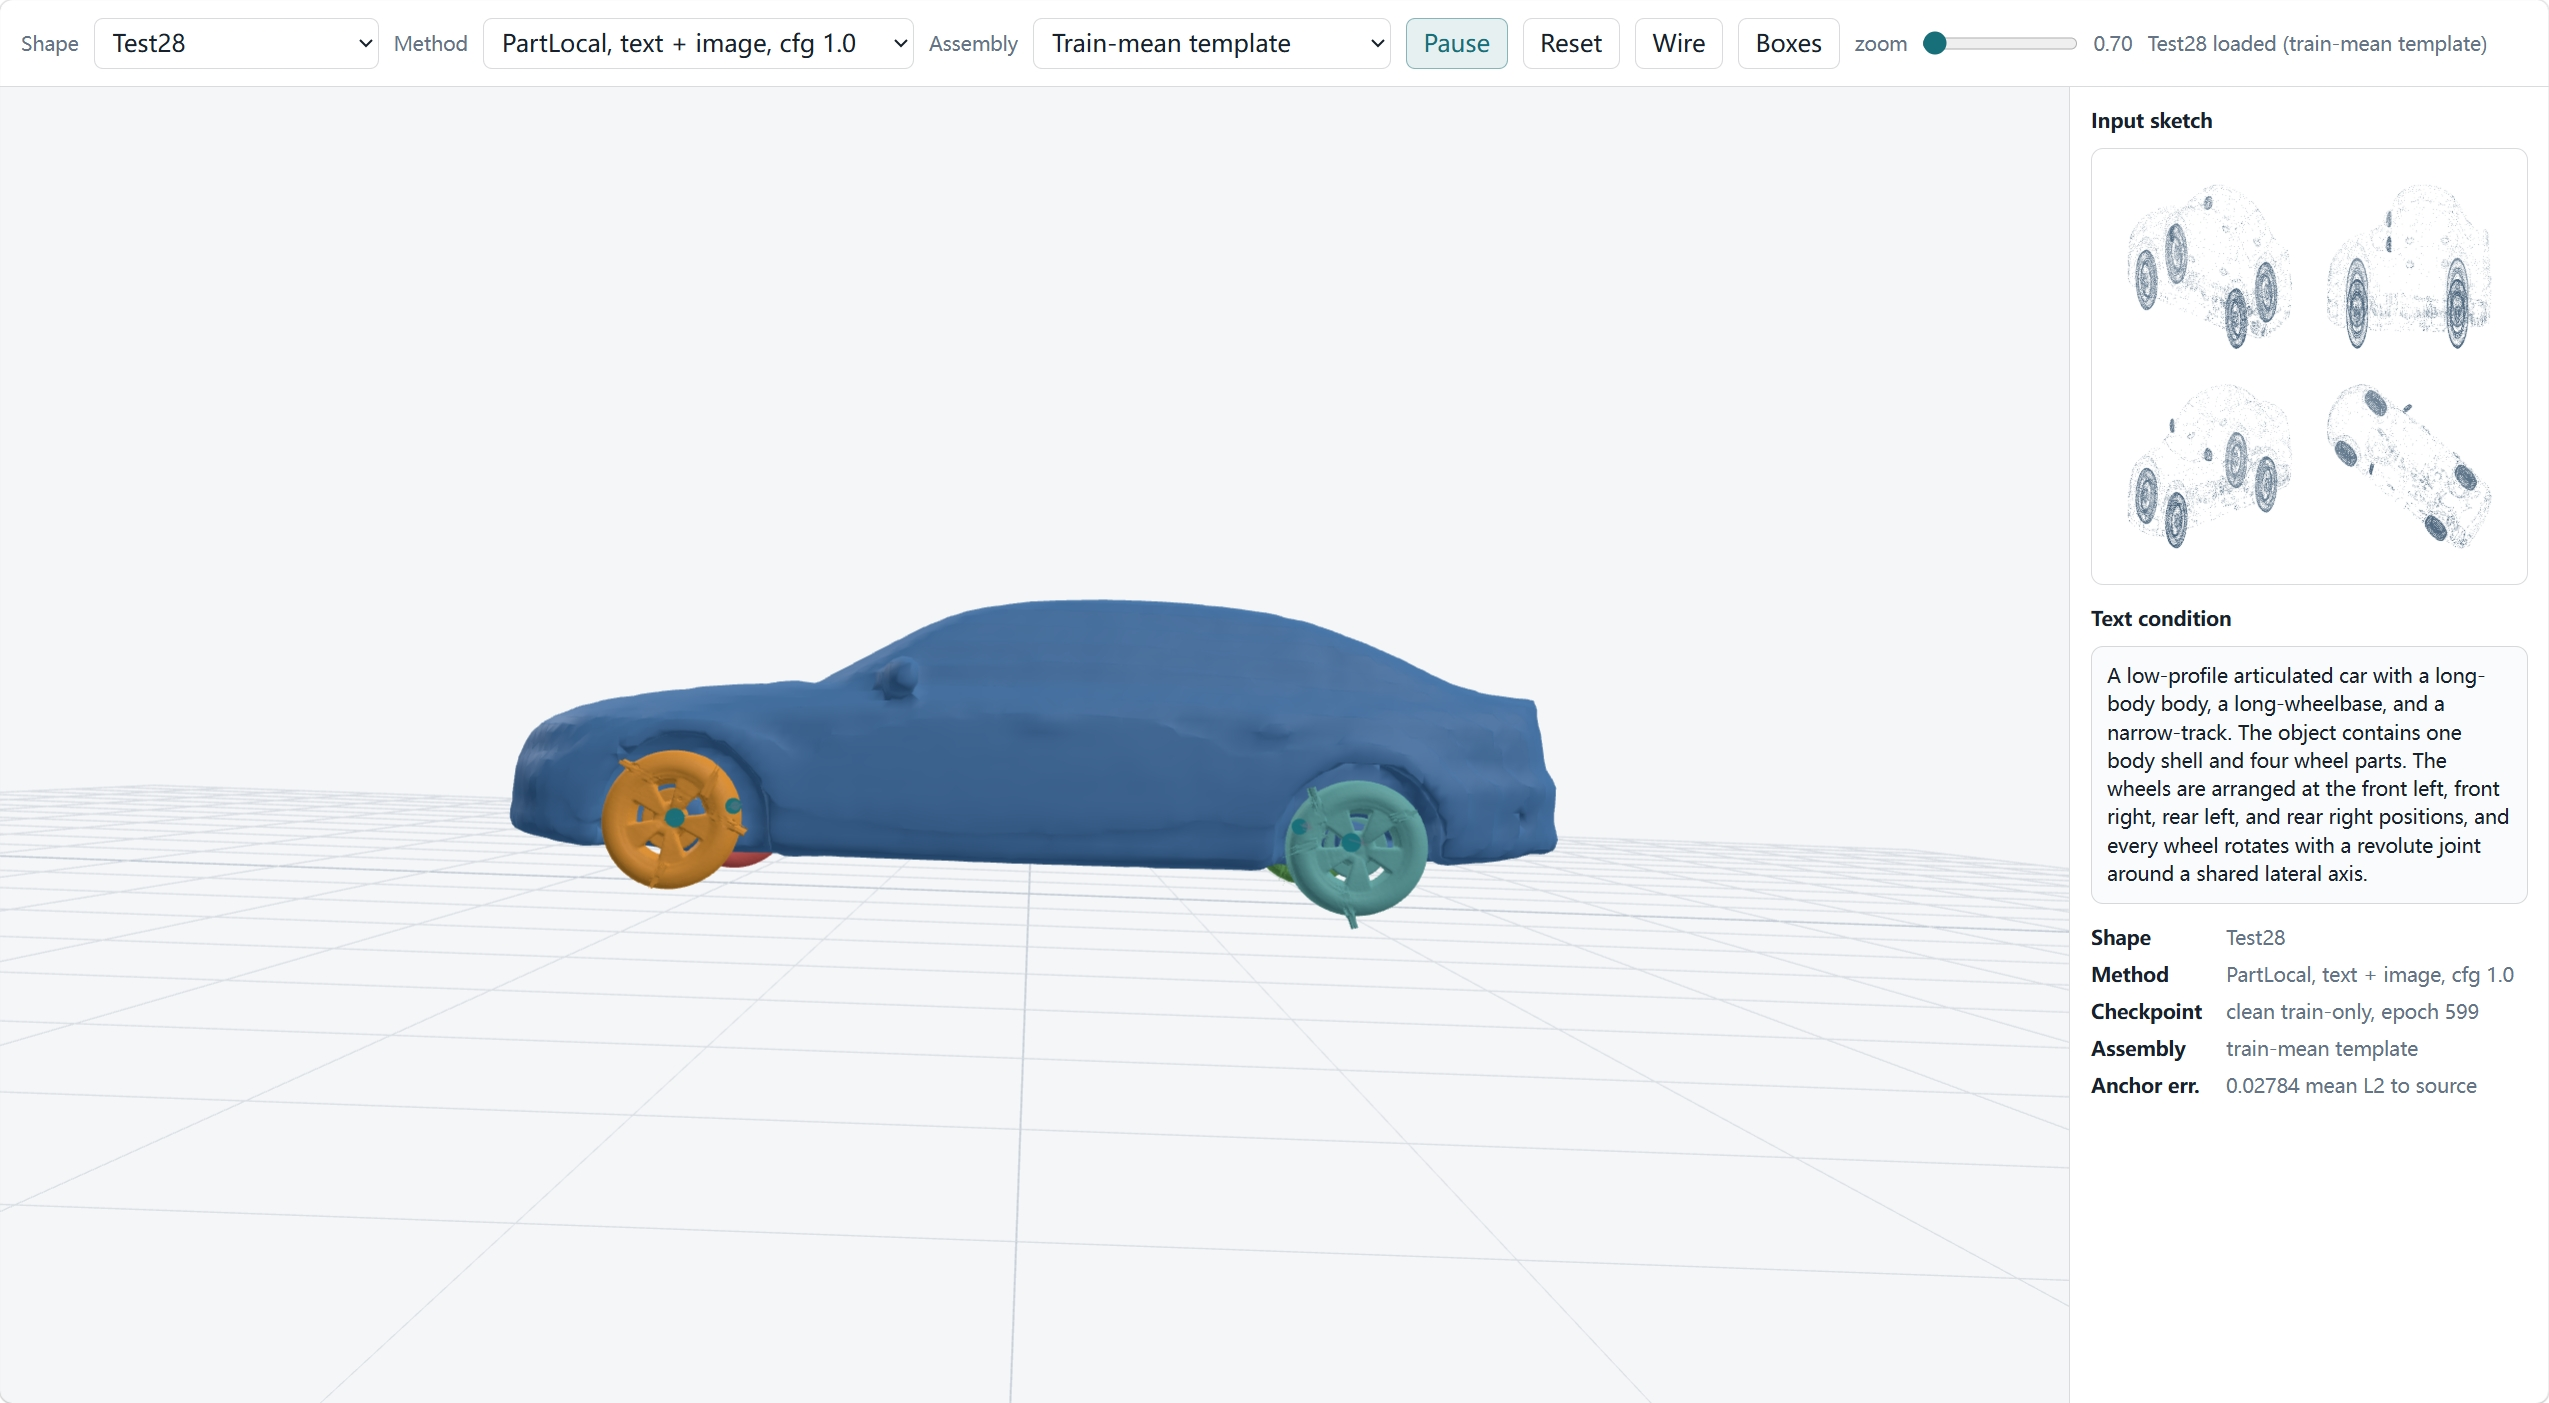
\includegraphics[width=0.46\linewidth]{LayoutNet_vs_ClassMean/classmean_28.jpeg} &
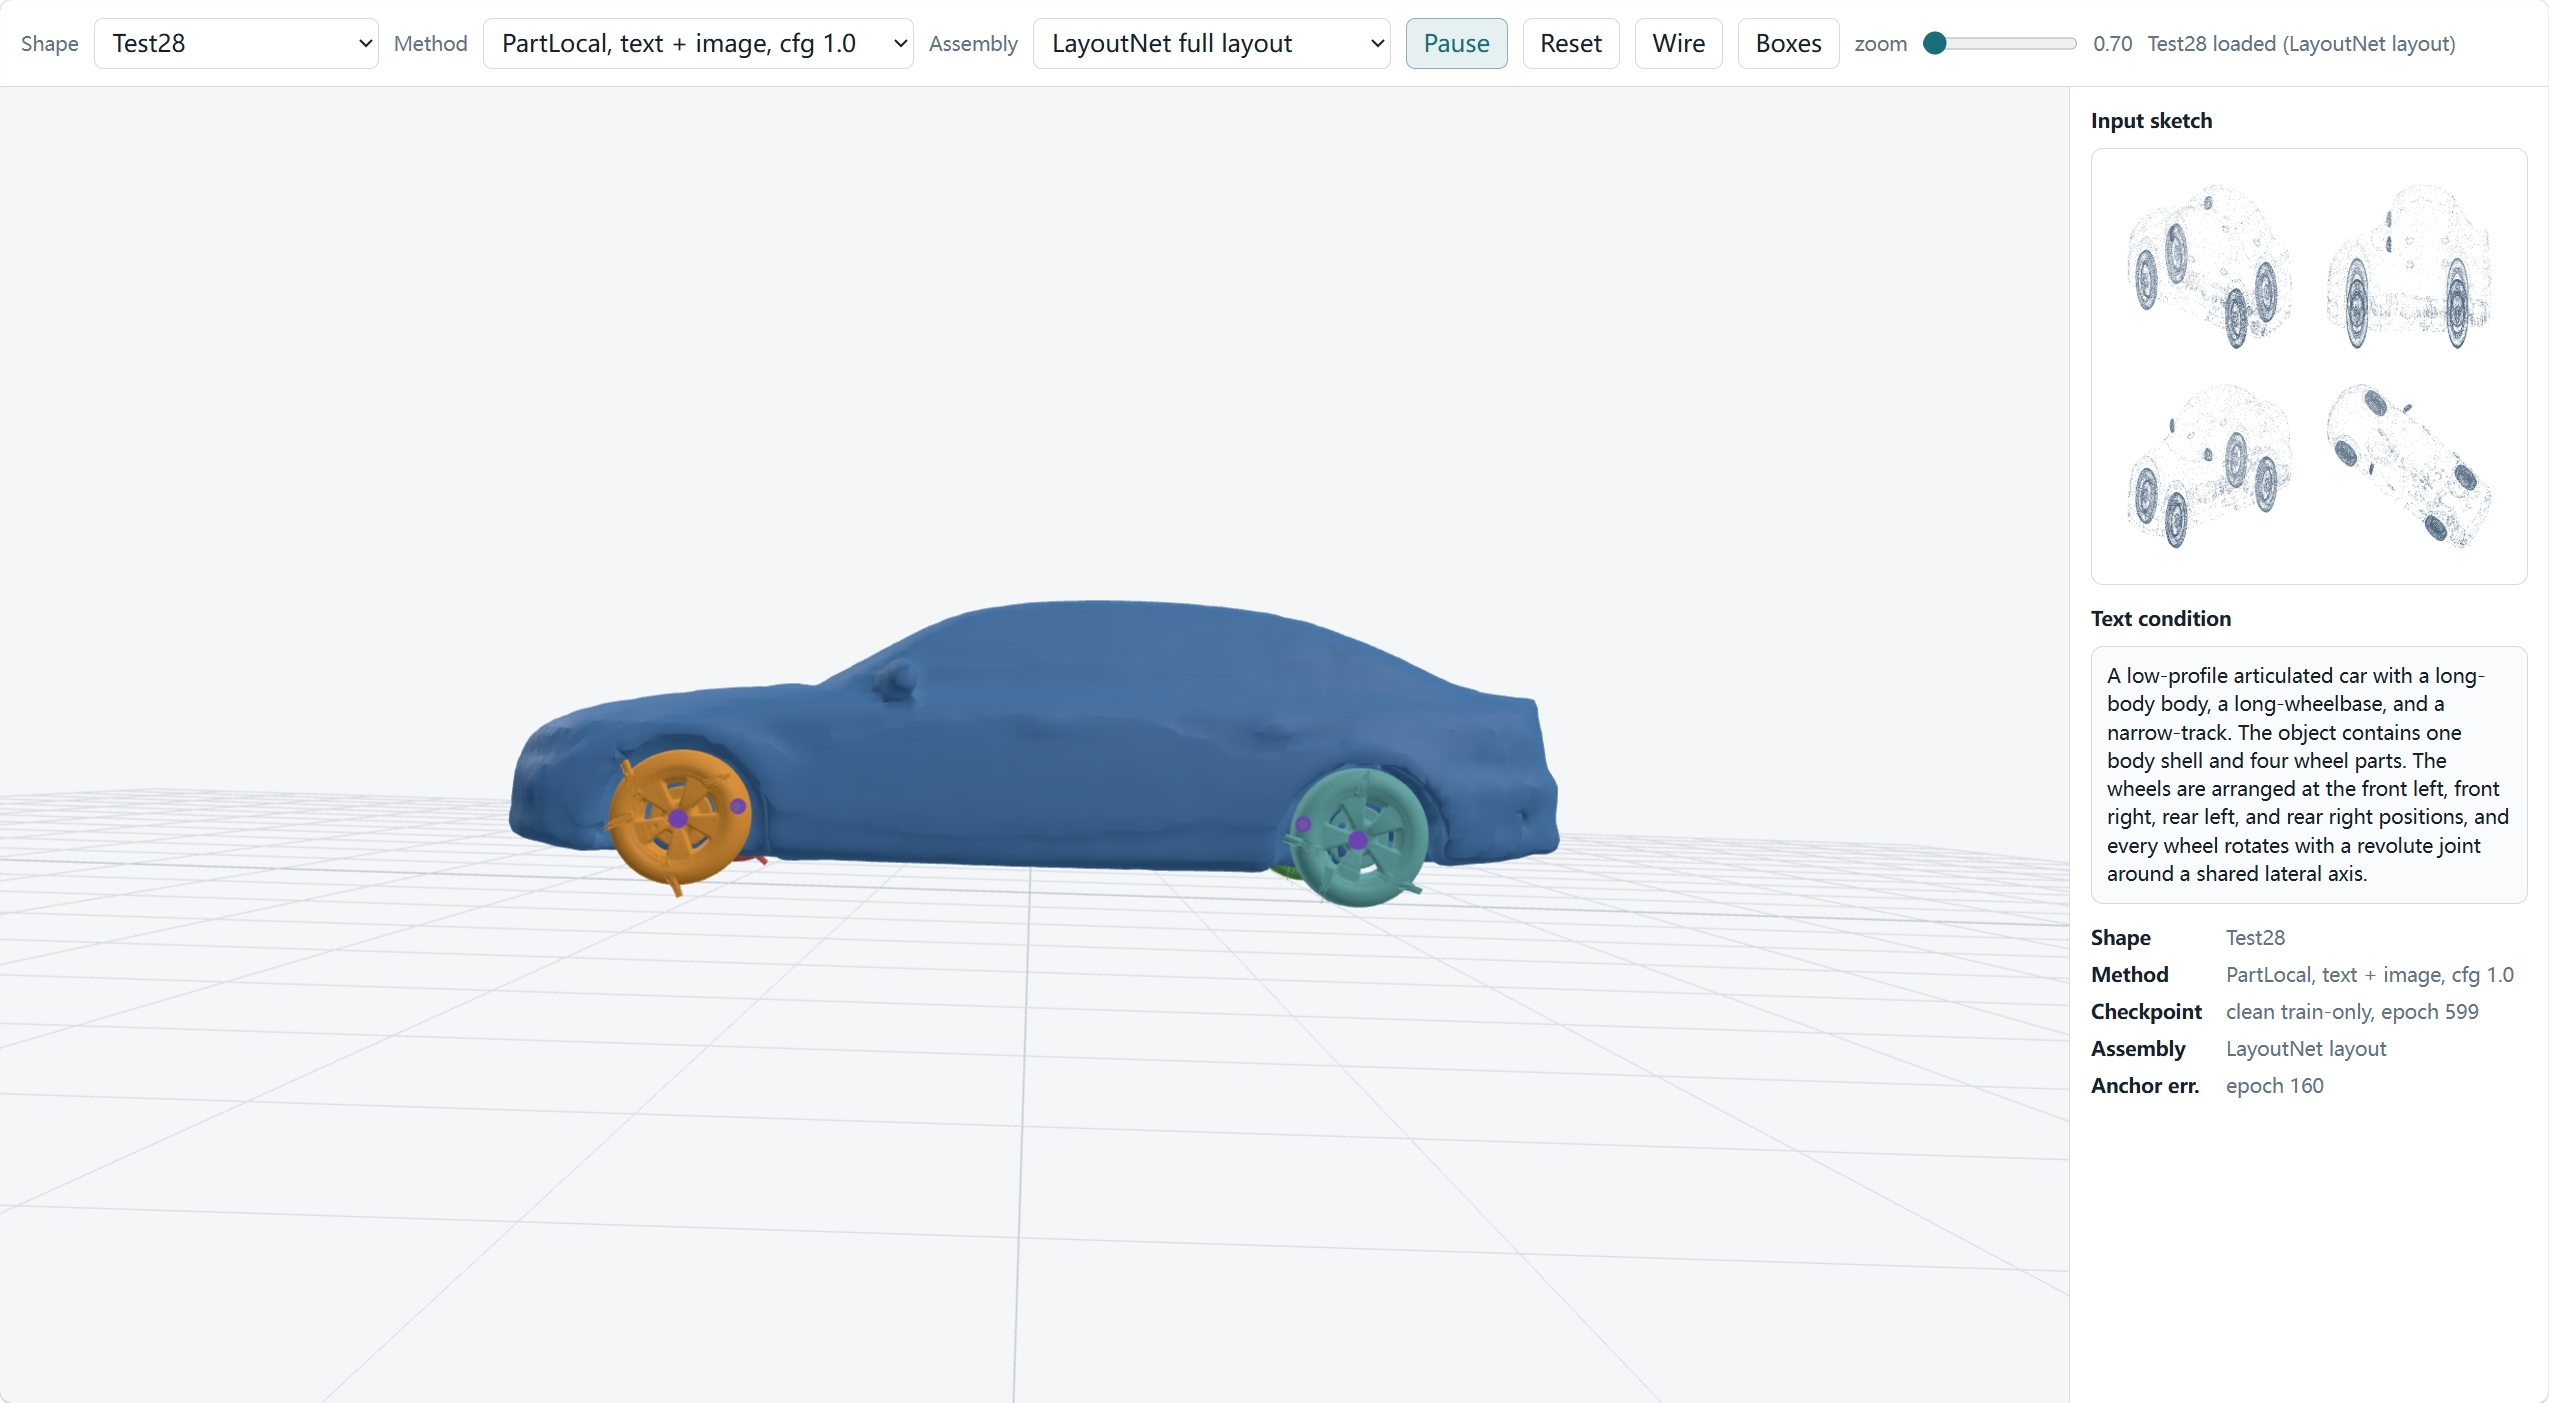
\includegraphics[width=0.46\linewidth]{LayoutNet_vs_ClassMean/LayoutNet_28.jpeg}
\end{tabular}
\caption{End-to-end assembly comparison without using a held-out source bounding box. LayoutNet gives more accurate wheel pivots and reduces the off-center wheel rotation visible in the ClassMean template.}
\label{fig:layout-comparison}
\end{figure}

\section{Limitations and Future Work}

\ 

We have to admit the dataset is too tiny. Only with 484 shapes, the model can learn the body-wheel
decomposition and basic design variation, but it cannot cover the full visual diversity of real vehicles. (I have to explain: we have found many datasets of vehicles with seperated parts, like Objaverse-XL and ShapeNet. However, I check each of them and find that their style is not realistic. Given that our goal is to generate realistic vehicle for downstream task like CFD, I decide to give up them temporarily.) Scaling the dataset
and improving text annotations is a important task in the future. 

CarActGen is currently limited to a fixed five-part car topology. This is useful for controlled study, but it does not cover vehicles with unusual wheel counts, openable doors, steering wheels, spoilers, mirrors, or internal mechanical parts. Extending the method to variable topology will require a large and high-quality dataset, a part-count generator or a graph-level structure module.

The current text module and sketch module is limited. The text module might encounter problems while facing unseen vocabulary and the sketch module can only deal with sketch with distinct ”DrivAerML-style”. I guess the limitations is also caused by our dataset.

Finally, the viewer is currently an evaluation and presentation tool rather than a full interactive system because of the limitations above. A stronger interactive system would allow users to edit prompts, sketch silhouettes, drag wheel positions, regenerate individual parts, and export assets to common 3D formats with animation metadata.

\section{Conclusion}

\

We introduced \method, a function-aware multimodal pipeline for generating structured four-wheel car assets. Starting from the \artformer articulated-object paradigm, we built a processed car dataset, redesigned the SDF VAE around function-aware latent conditioning, replaced routed multimodal diffusion with a PartLocal object denoiser, and added LayoutNet for functional assembly. Our clean split audit shows that the main value of the new VAE is not raw reconstruction superiority, but a better plane-feature interface for diffusion. It also makes the diffusion result more honest: PartLocal improves body geometry under joint text--image conditioning, but neither the clean original baseline nor the clean PartLocal rerun yet satisfies strict watertight wheel validity. Finally, LayoutNet turns fixed template assembly into a measurable baseline and substantially improves held-out box and pivot prediction. The remaining challenges are clear: wheel geometry is still hard, the topology is fixed, and richer local visual supervision is needed for more faithful interactable vehicle assets.

\begin{thebibliography}{99}

\bibitem{artformer2025}
J. Su, Y. Feng, Z. Li, J. Song, Y. He, B. Ren, and B. Xu.
\newblock ArtFormer: Controllable Generation of Diverse 3D Articulated Objects.
\newblock In \emph{Proceedings of the IEEE/CVF Conference on Computer Vision and Pattern Recognition (CVPR)}, 2025.

\bibitem{drivaerml2024}
N. Ashton, C. Mockett, M. Fuchs, L. Fliessbach, H. Hetmann, T. Knacke, N. Schönwald, V. Skaperdas, G. Fotiadis, A. Walle, B. Hupertz, and D. C. Maddix.
\newblock DrivAerML: High-Fidelity Computational Fluid Dynamics Dataset for Road-Car External Aerodynamics.
\newblock arXiv preprint arXiv:2408.11969, 2024.

\bibitem{park2019deepsdf}
J. J. Park, P. Florence, J. Straub, R. Newcombe, and S. Lovegrove.
\newblock DeepSDF: Learning Continuous Signed Distance Functions for Shape Representation.
\newblock In \emph{CVPR}, 2019.

\bibitem{mescheder2019occupancy}
L. Mescheder, M. Oechsle, M. Niemeyer, S. Nowozin, and A. Geiger.
\newblock Occupancy Networks: Learning 3D Reconstruction in Function Space.
\newblock In \emph{CVPR}, 2019.

\bibitem{chou2022gensdf}
G. Chou, I. Chugunov, and F. Heide.
\newblock GenSDF: Two-Stage Learning of Generalizable Signed Distance Functions.
\newblock In \emph{NeurIPS}, 2022.

\bibitem{ho2020ddpm}
J. Ho, A. Jain, and P. Abbeel.
\newblock Denoising Diffusion Probabilistic Models.
\newblock In \emph{NeurIPS}, 2020.

\bibitem{song2020ddim}
J. Song, C. Meng, and S. Ermon.
\newblock Denoising Diffusion Implicit Models.
\newblock In \emph{ICLR}, 2021.

\bibitem{perez2018film}
E. Perez, F. Strub, H. de Vries, V. Dumoulin, and A. Courville.
\newblock FiLM: Visual Reasoning with a General Conditioning Layer.
\newblock In \emph{AAAI}, 2018.

\bibitem{raffel2020t5}
C. Raffel, N. Shazeer, A. Roberts, K. Lee, S. Narang, M. Matena, Y. Zhou, W. Li, and P. J. Liu.
\newblock Exploring the Limits of Transfer Learning with a Unified Text-to-Text Transformer.
\newblock \emph{Journal of Machine Learning Research}, 21(140):1--67, 2020.

\bibitem{oquab2023dinov2}
M. Oquab, T. Darcet, T. Moutakanni, H. Vo, M. Szafraniec, V. Khalidov, P. Fernandez, D. Haziza, F. Massa, A. El-Nouby, and collaborators.
\newblock DINOv2: Learning Robust Visual Features without Supervision.
\newblock \emph{Transactions on Machine Learning Research}, 2024.

\bibitem{xiang2020sapien}
F. Xiang, Y. Qin, K. Mo, Y. Xia, H. Zhu, F. Liu, M. Liu, H. Jiang, Y. Yuan, H. Wang, and collaborators.
\newblock SAPIEN: A SimulAted Part-based Interactive ENvironment.
\newblock In \emph{CVPR}, 2020.

\bibitem{mo2019partnet}
K. Mo, S. Zhu, A. X. Chang, L. Yi, S. Tripathi, L. J. Guibas, and H. Su.
\newblock PartNet: A Large-scale Benchmark for Fine-grained and Hierarchical Part-level 3D Object Understanding.
\newblock In \emph{CVPR}, 2019.

\bibitem{poole2022dreamfusion}
B. Poole, A. Jain, J. T. Barron, and B. Mildenhall.
\newblock DreamFusion: Text-to-3D using 2D Diffusion.
\newblock In \emph{ICLR}, 2023.

\bibitem{lin2023magic3d}
C.-H. Lin, J. Gao, L. Tang, T. Takikawa, X. Zeng, X. Huang, K. Kreis, S. Fidler, M.-Y. Liu, and T.-Y. Lin.
\newblock Magic3D: High-Resolution Text-to-3D Content Creation.
\newblock In \emph{CVPR}, 2023.

\bibitem{nichol2022point-e}
A. Nichol, H. Jun, P. Dhariwal, P. Mishkin, and M. Chen.
\newblock Point-E: A System for Generating 3D Point Clouds from Complex Prompts.
\newblock arXiv preprint arXiv:2212.08751, 2022.

\bibitem{jun2023shap-e}
H. Jun and A. Nichol.
\newblock Shap-E: Generating Conditional 3D Implicit Functions.
\newblock arXiv preprint arXiv:2305.02463, 2023.

\end{thebibliography}

\end{document}
